\documentclass[a4paper,9pt]{extarticle}
\usepackage[ngerman]{babel}
\usepackage{amsmath,amsthm}
\usepackage{ascii}
\usepackage[adobe-utopia]{mathdesign}
\usepackage[T1]{fontenc}
\usepackage[margin=0.1cm]{geometry}
\usepackage{multicol}
\usepackage{color,graphicx,overpic}
\usepackage{hyperref}
%Enumerator
\usepackage[inline]{enumitem}
%Table imports
\newcommand{\ra}[1]{\renewcommand{\arraystretch}{#1}}
%Style imports
\usepackage{enumitem}
\usepackage{tcolorbox}
\usepackage{listings}
\usepackage{minted}
\usepackage{algorithm}
\usepackage{algpseudocode}
\usepackage{authblk}
\usepackage{fancyhdr}
\usepackage{fancyhdr}
\usepackage{datetime}
\usepackage[iso,german]{isodate}
%Graphic imports
\usepackage{tikz}
\graphicspath{ {./img/} }
% Turn off header and footer
\pagestyle{empty}

% Redefine section commands to use less space
\makeatletter
\renewcommand{\section}{\@startsection{section}{1}{0mm}%
                                {-1ex plus -.5ex minus -.2ex}%
                                {0.5ex plus .2ex}%x
                                {\normalfont\large\bfseries}}
\renewcommand{\subsection}{\@startsection{subsection}{2}{0mm}%
                                {-1explus -.5ex minus -.2ex}%
                                {0.5ex plus .2ex}%
                                {\normalfont\normalsize\bfseries}}
\renewcommand{\subsubsection}{\@startsection{subsubsection}{3}{0mm}%
                                {-1ex plus -.5ex minus -.2ex}%
                                {1ex plus .2ex}%
                                {\normalfont\small\bfseries}}
\renewcommand{\paragraph}{%
  \@startsection{paragraph}{4}%
  {\z@}{1ex \@plus 1ex \@minus .2ex}{-1em}%
  {\normalfont\normalsize\bfseries}%
}
\makeatother

% Define BibTeX command
\def\BibTeX{{\rm B\kern-.05em{\sc i\kern-.025em b}\kern-.08em
    T\kern-.1667em\lower.7ex\hbox{E}\kern-.125emX}}

% Don't print section numbers
\setcounter{secnumdepth}{0}

\setlength{\parindent}{0pt}
\setlength{\parskip}{0pt plus 0.5ex}

%My Environments
\newtheorem{example}[section]{Example}
% -----------------------------------------------------------------------
\definecolor{codegreen}{rgb}{0,0.6,0}
\definecolor{codegray}{rgb}{0.5,0.5,0.5}
\definecolor{codepurple}{rgb}{0.58,0,0.82}
\definecolor{backcolour}{rgb}{0.95,0.95,0.92}
\lstdefinelanguage{CSS}{
  morekeywords={accelerator,azimuth,background,background-attachment,
    background-color,background-image,background-position,
    background-position-x,background-position-y,background-repeat,
    behavior,border,border-bottom,border-bottom-color,
    border-bottom-style,border-bottom-width,border-collapse,
    border-color,border-left,border-left-color,border-left-style,
    border-left-width,border-right,border-right-color,
    border-right-style,border-right-width,border-spacing,
    border-style,border-top,border-top-color,border-top-style,
    border-top-width,border-width,bottom,caption-side,clear,
    clip,color,content,counter-increment,counter-reset,cue,
    cue-after,cue-before,cursor,direction,display,elevation,
    empty-cells,filter,float,font,font-family,font-size,
    font-size-adjust,font-stretch,font-style,font-variant,
    font-weight,height,ime-mode,include-source,
    layer-background-color,layer-background-image,layout-flow,
    layout-grid,layout-grid-char,layout-grid-char-spacing,
    layout-grid-line,layout-grid-mode,layout-grid-type,left,
    letter-spacing,line-break,line-height,list-style,
    list-style-image,list-style-position,list-style-type,margin,
    margin-bottom,margin-left,margin-right,margin-top,
    marker-offset,marks,max-height,max-width,min-height,
    min-width,-moz-binding,-moz-border-radius,
    -moz-border-radius-topleft,-moz-border-radius-topright,
    -moz-border-radius-bottomright,-moz-border-radius-bottomleft,
    -moz-border-top-colors,-moz-border-right-colors,
    -moz-border-bottom-colors,-moz-border-left-colors,-moz-opacity,
    -moz-outline,-moz-outline-color,-moz-outline-style,
    -moz-outline-width,-moz-user-focus,-moz-user-input,
    -moz-user-modify,-moz-user-select,orphans,outline,
    outline-color,outline-style,outline-width,overflow,
    overflow-X,overflow-Y,padding,padding-bottom,padding-left,
    padding-right,padding-top,page,page-break-after,
    page-break-before,page-break-inside,pause,pause-after,
    pause-before,pitch,pitch-range,play-during,position,quotes,
    -replace,richness,right,ruby-align,ruby-overhang,
    ruby-position,-set-link-source,size,speak,speak-header,
    speak-numeral,speak-punctuation,speech-rate,stress,
    scrollbar-arrow-color,scrollbar-base-color,
    scrollbar-dark-shadow-color,scrollbar-face-color,
    scrollbar-highlight-color,scrollbar-shadow-color,
    scrollbar-3d-light-color,scrollbar-track-color,table-layout,
    text-align,text-align-last,text-decoration,text-indent,
    text-justify,text-overflow,text-shadow,text-transform,
    text-autospace,text-kashida-space,text-underline-position,top,
    unicode-bidi,-use-link-source,vertical-align,visibility,
    voice-family,volume,white-space,widows,width,word-break,
    word-spacing,word-wrap,writing-mode,z-index,zoom},
  morestring=[s]{:}{;},
  sensitive,
  morecomment=[s]{/*}{*/}
}
%=====================================SCSS=========================================
\lstdefinelanguage{SCSS}{
    morekeywords={accelerator,azimuth,background,background-attachment,
    background-color,background-image,background-position,
    background-position-x,background-position-y,background-repeat,
    behavior,border,border-bottom,border-bottom-color,
    border-bottom-style,border-bottom-width,border-collapse,
    border-color,border-left,border-left-color,border-left-style,
    border-left-width,border-right,border-right-color,
    border-right-style,border-right-width,border-spacing,
    border-style,border-top,border-top-color,border-top-style,
    border-top-width,border-width,bottom,caption-side,clear,
    clip,color,content,counter-increment,counter-reset,cue,
    cue-after,cue-before,cursor,direction,display,elevation,
    empty-cells,filter,float,font,font-family,font-size,
    font-size-adjust,font-stretch,font-style,font-variant,
    font-weight,height,ime-mode,include-source,
    layer-background-color,layer-background-image,layout-flow,
    layout-grid,layout-grid-char,layout-grid-char-spacing,
    layout-grid-line,layout-grid-mode,layout-grid-type,left,
    letter-spacing,line-break,line-height,list-style,
    list-style-image,list-style-position,list-style-type,margin,
    margin-bottom,margin-left,margin-right,margin-top,
    marker-offset,marks,max-height,max-width,min-height,
    min-width,-moz-binding,-moz-border-radius,
    -moz-border-radius-topleft,-moz-border-radius-topright,
    -moz-border-radius-bottomright,-moz-border-radius-bottomleft,
    -moz-border-top-colors,-moz-border-right-colors,
    -moz-border-bottom-colors,-moz-border-left-colors,-moz-opacity,
    -moz-outline,-moz-outline-color,-moz-outline-style,
    -moz-outline-width,-moz-user-focus,-moz-user-input,
    -moz-user-modify,-moz-user-select,orphans,outline,
    outline-color,outline-style,outline-width,overflow,
    overflow-X,overflow-Y,padding,padding-bottom,padding-left,
    padding-right,padding-top,page,page-break-after,
    page-break-before,page-break-inside,pause,pause-after,
    pause-before,pitch,pitch-range,play-during,position,quotes,
    -replace,richness,right,ruby-align,ruby-overhang,
    ruby-position,-set-link-source,size,speak,speak-header,
    speak-numeral,speak-punctuation,speech-rate,stress,
    scrollbar-arrow-color,scrollbar-base-color,
    scrollbar-dark-shadow-color,scrollbar-face-color,
    scrollbar-highlight-color,scrollbar-shadow-color,
    scrollbar-3d-light-color,scrollbar-track-color,table-layout,
    text-align,text-align-last,text-decoration,text-indent,
    text-justify,text-overflow,text-shadow,text-transform,
    text-autospace,text-kashida-space,text-underline-position,top,
    unicode-bidi,-use-link-source,vertical-align,visibility,
    voice-family,volume,white-space,widows,width,word-break,
    word-spacing,word-wrap,writing-mode,z-index,zoom},
    comment=[l]{//},
    ndkeywords = {@mixin}
}
%==================================Javascript======================================
\lstdefinelanguage{JavaScript}{
  keywords={typeof, new, true, false, catch, function, return, null, catch, switch, var, if, in, while, do, else, case, break},
  ndkeywords={class, export, boolean, throw, implements, import, this},
  sensitive=false,
  comment=[l]{//},
  morecomment=[s]{/*}{*/},
  morestring=[b]',
  morestring=[b]"
}
\lstdefinestyle{sharpc}{language=[Sharp]C}
\lstset{aboveskip=2pt,belowskip=3pt}
\lstset{ %
    backgroundcolor=\color{backcolour},   
    commentstyle=\color{codegreen},
    keywordstyle=\color{magenta},
    numberstyle=\tiny\color{codegray},
    stringstyle=\color{codepurple},
    basicstyle=\scriptsize,
    breakatwhitespace=false,         
    breaklines=true,                 
    captionpos=b,                    
    keepspaces=true,                 
    numbers=none,                    
    numbersep=5pt,                  
    showspaces=false,                
    showstringspaces=false,
    showtabs=false,                  
    tabsize=2,
    frame=single,
    language=[Sharp]C,
    postbreak=\raisebox{0ex}[0ex][0ex]{\ensuremath{\color{black}\hookrightarrow\space}}
}
\algrenewcommand\algorithmicfunction{\textbf{algorithm}}
\newcommand{\code}[1]{\texttt{#1}}
\title{Mobile and GUI Engineering\\\Large WPF}
\author{Severin Dellsperger \\ Julian Klaiber}
\date{Herbstsemester 2019}
\affil{Hochschule für Technik Rapperswil}
\begin{document}
\raggedright
\footnotesize
\begin{multicols*}{3}

% multicol parameters
% These lengths are set only within the two main columns
%\setlength{\columnseprule}{0.25pt}
\setlength{\premulticols}{1pt}
\setlength{\postmulticols}{1pt}
\setlength{\multicolsep}{1pt}
\setlength{\columnsep}{2pt}
\section{Grundlagen der GUI Programmierung}
Apps bestehen aus lose gekoppelten, wiederverwendbaren Komponenten. Diese sind Activities (für den Benutzer sichtbar) und Services, Content Provider, Broadcast Receivers (unsichtbar für Benutzer). \textbf{Erbt nicht von Context und Fragment ist keine Komponente}. Das System hat die Kontrolle über alle Applikationen und Verwaltet den Lebenszyklus, ist verantwortlich für die Kommunikation zwischen Komponenten und schliesst die Apps automatisch um Speicher zu sparen.
\paragraph{Activites} Dies sind die \textbf{Hauptbausteine} in der App Entwicklung, die Activity interagiert mit dem Benutzer. Eine Activity stellt immer auch einen möglichen Eintrittspunkt in die App ein. Bei einem Wechsel in einen anderen Zustand des Lebenszyklus wird die betroffene Activity über einen Methodenaufruf informiert.

\textbf{Activity = Gui + Code}
\begin{lstlisting}[language=java]
public class MainActivity extends Activity {
  @Override
  protected void onCreate(Bundle savedInstanceState) {
    super.onCreate(savedInstanceState);
    /* Hier unser Code z.B
    setContentView(R.layout.activity_main);*/
  }
}
\end{lstlisting}
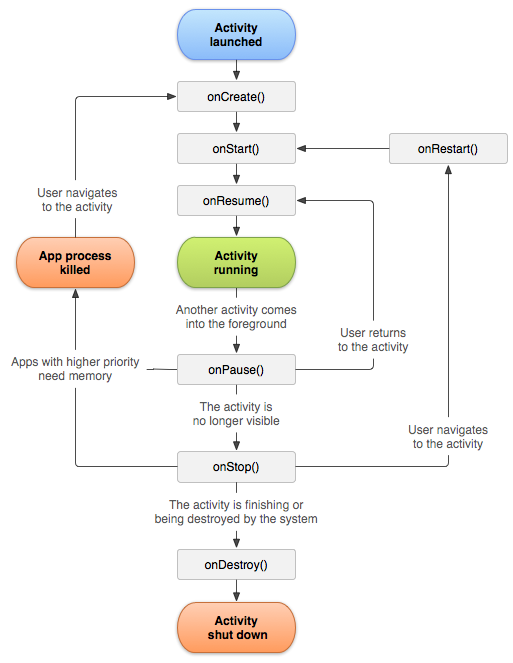
\includegraphics[scale=0.35]{activity_lifecycle.png}
Unterschied Paused/Resume: wird die Activity von einer anderen überdeckt (z.B. Notificationleiste heruntergezogen), wird die erste pausiert (\code{onPause}). Kommt sie wieder in den Vordergrund, wird wieder \code{onResume} aufgerufen.

\code{onPause} ist \textbf{garantiert}. \code{onStop} ist jedoch \textbf{nicht garantiert}. Darum:

\paragraph{Best Practice}

\begin{itemize}
  \item \code{onCreate} erstellt GUI beim Start.
  \item \code{onResume} reagiert auf Benutzereingaben.
  \item \code{onPause} sichert Daten (da die App auch im \code{onStop} oder \code{onDestroy} gekillt werden kann).
  \item \code{onStop} gibt Ressourcen frei.
\end{itemize}

Bei Konfigurationsänderungen wird die Activity neu gestartet. Dazu zählen z.B. \textbf{Screenausrichtungsänderungen}.

\textbf{Stopped/Started:} kommt die Activity wieder in den Vordergrund, weil der User die Applikation nochmal startet oder mit dem Back-Button zurückkommt, wird onRestart() aufgerufen.

\textbf{Destroyed}: die App wird vom System destroyed, oder wenn sie explizit vom User geschlossen wird.

\paragraph{Activity Stack}

Activities werden in einem Stack verwaltet, wobei die Activites eines Stacks zu verschiedenen Apps gehören können.\\ 
Eine \textbf{Gruppe von Activities} in einem Stack nennt man auch \textbf{Task}. Es können mehrere Tasks gleichzeitig existieren. Tasks lassen sich im Overview Screen anzeigen.

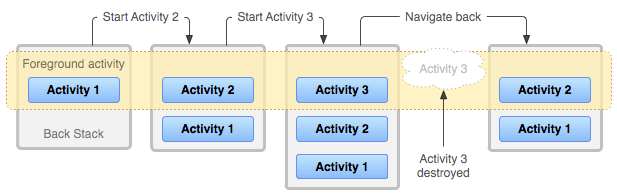
\includegraphics[scale=0.29]{diagram_backstack.png}


\paragraph{APK}

Activities (und Ressourcen, etc) werden in ein APK gepackt und installiert. Wird eine Activity aktiv, wird pro APK ein Linux Prozess mit einem Thread gestartet, welcher alle Activities die indiesem APK enthalten sind ausführt. Jedes APK wird unter einem eigenen Linux-User installiert. Inhalt: Libraries, Ressourcen, Assets, Metadaten, kompilierte Klassen im DEX-Format.

Ein APK ist nichts anderes als ein JAR, welches wiederum eine ZIP-Datei ist.
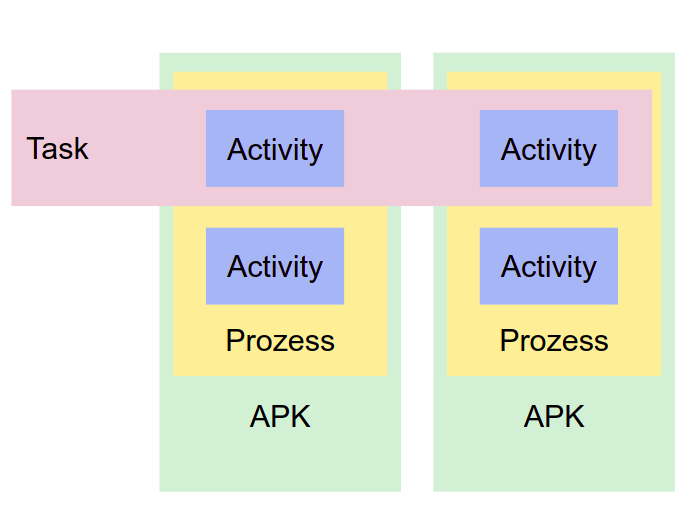
\includegraphics[scale=0.20]{img/activities-tasks-systemsicht.png}

\subsection{Application}
Parent unserer Activities im Manifest ist die Application. Ist auch eine Klasse, die den globalen Zustand unserer App hält. Kann durch eigene Application-Subklasser ersetzt werden. Zugriff aus Activity mit \code{getApplication}, Lifecycle-Methoden: \code{onCreate}, \code{onLowMemory}, \code{onConfigurationChanged}.

\paragraph{Bundle}
Bundles werden in der Regel für den Datenaustausch zwischen verschiedenen Android-Aktivitäten verwendet. Bundles können alle Arten von Werten enthalten und an die neue Aktivität übergeben.

\paragraph{Intent}
\textbf{Kommunikation zwischen Komponenten (Activities, Services, Broadcasts)}
Ein Intent beschreibt was gemacht werden soll \\
- \textbf{Explizit} - Aufruf der Klasse \\
-  \textbf{Implizit} - Aufruf passender Komponente (System entscheidet - geeignet für Systemapps z.B Foto).\\
Apps können selbst wiederum Activites zur Verfügung stellen und bestehende Applikationen ersetzen.
\begin{lstlisting}[language=java]
// Explizit mit Klasse
Intent in = new Intent(this, CalculateActivity.class)
// Implizit mit Aktion z.B Bild erstellen 
Intent in = new Intent(MediaStore.ACTION_IMAGE_CAPUTRE)
\end{lstlisting}
Andere Activities kann man mit \code{startActivity(intent)} oder \code{startActivityForResult(intent, myId)} starten (Resultat wird über Callback kommuniziert und Activity wird nicht blockiert). Um bei letzterem mit dem Rückgabewert arbeiten zu können muss man \code{onActivityResult} überschreiben.
\begin{lstlisting}[language=java]
@Override
protected void onActivityResult(int request, int result, Intent data) {
  if (result == Activity.RESULT_OK && request == myId) {
    /* Resultat verarbeiten */
  }
}
\end{lstlisting}
\begin{lstlisting}[language=java]
//Einfacher Intent aus onCreate Methode
@Override
protected void onCreate(Bundle savedInstanceState) {
    super.onCreate(savedInstanceState);
    setContentView(R.layout.activity_main);

    // einfacher Intent
    final Button button = (Button) findViewById(R.id.btn);
    button.setOnClickListener(new View.OnClickListener() {
        @Override
        public void onClick(View v) {
           Intent it = new Intent(MainActivity.this, SecondActivity.class);
           startActivity(it);
        }
    });
\end{lstlisting}
Möchte man einem Intent Daten übergeben, kann man das entweder mit der \code{setData} Methode, welche eine URI entgegennimmt, oder mit \code{in.putExtra(MediaStore.EXTRA\_OUTPUT, imageCaptureUri)}. Letzere ist eine Struktur mit Key-Value Paaren und nimmt nur primitive Daten, Strings und serialisierbare Datentypen an.
\begin{lstlisting}[language=java]
public class MainActivity extends Activity {

    @Override
    protected void onCreate(Bundle savedInstanceState) {
        super.onCreate(savedInstanceState);
        setContentView(R.layout.activity_main);

        // Intent mit Werten zu arbeiten
        final Button button = (Button) findViewById(R.id.btn);
        button.setOnClickListener(new View.OnClickListener() {
            @Override
            public void onClick(View v) {
               final int myId = 99;
               Intent it = new Intent(MainActivity.this, SecondActivity.class);
               it.putExtra("name", "severin" ); //key value Attribute uebergeben
               startActivityForResult(it, myId); // Activity mit Result starten
            }
        });
    }
    @Override // Activity mit Result auswerten
    protected void onActivityResult(int request, int result, Intent data) {
        if(result == Activity.RESULT_OK && request == 99)
        {
            findViewById(R.id.btn).setEnabled(false);

        }

    }
}

public class SecondActivity extends Activity {

    static final int myId = 99;

    @Override
    protected void onCreate(Bundle savedInstanceState) {
        super.onCreate(savedInstanceState);
        setContentView(R.layout.activity_second);

        TextView txt = findViewById(R.id.txt);
        // Intent Daten/Extras auswerten
        Bundle extras = getIntent().getExtras(); 
        txt.setText(extras.getString("name"));

        final Button button = (Button) findViewById(R.id.btn);
        button.setOnClickListener(new View.OnClickListener() {
            @Override
            public void onClick(View v) {
                // Neuen Intent mit Result erstellen/zurücksenden
                Intent returnIntent = new Intent();
                returnIntent.putExtra("result", "Result OK");
                setResult(Activity.RESULT_OK, returnIntent);
                finish();
            }

        });
    }
}

\end{lstlisting}


\paragraph{Manifest} Das Manifest enthält Meta-Daten einer App. Es umfasst
\begin{itemize}
\item Komponenten der App
\item Metadaten (Name, Icon, Versionsnummer)
\item Permissions (Internet, kostenpflichtige Anrufe etc.)
\item Anforderungen an die Geräte API
\item \code{minSdkVersion} min-Version des Gerätes
\item \code{targetSdkVersion} höchste Version, mit der getestet wurde
\item \textbf{Name der Singleton Instanz der Application (Sub-)Klasse.}
\end{itemize}

Das Manifest wird vom System verwendet um zu wissen, ob die App installiert werden kann, welche Permissions diese verwendet etc.
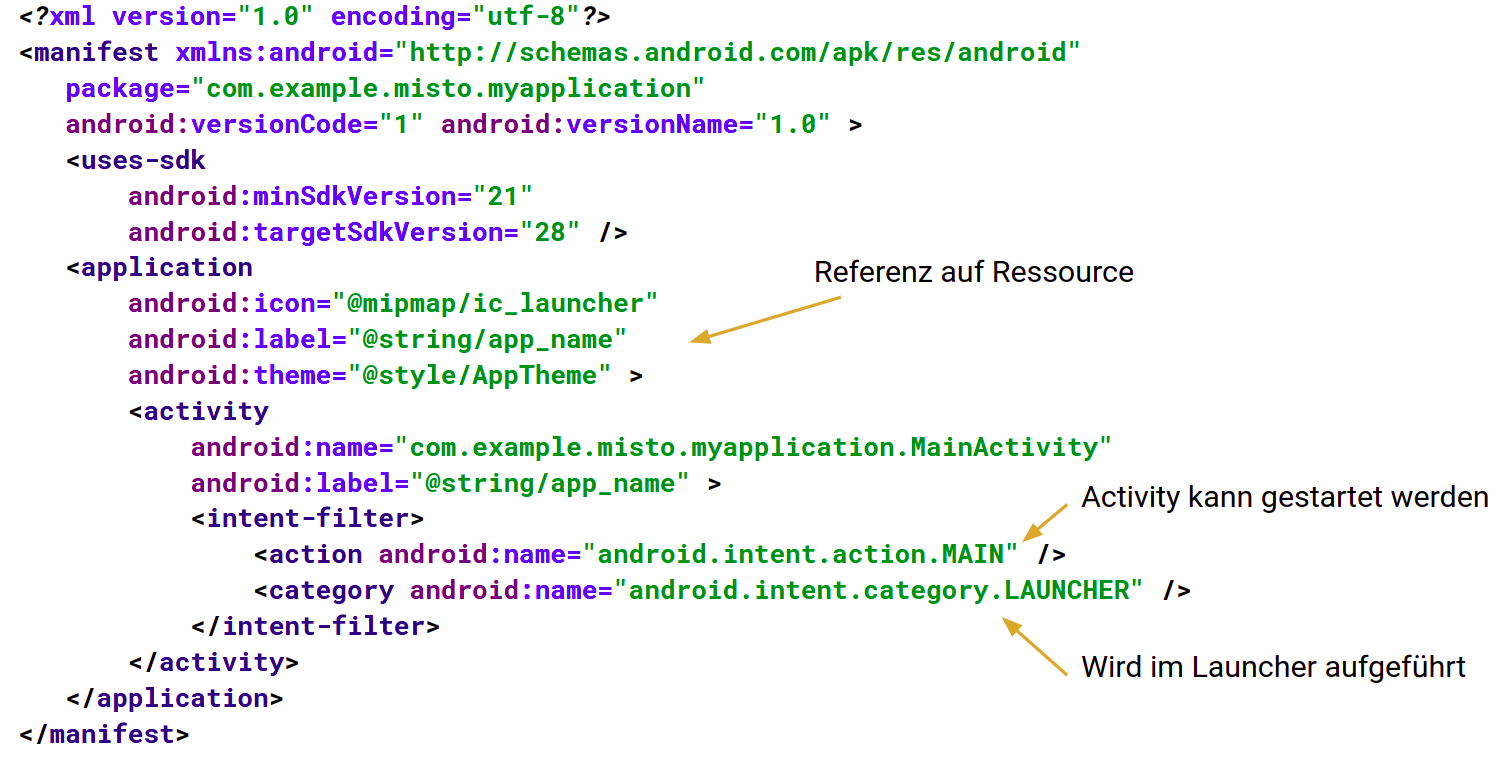
\includegraphics[scale=0.17]{img/manifest.png}

\subsection{Android GUI}
\paragraph{View} Die Basisklasse um User Interfaces zu bauen ist die \code{View}. Eine View ist zuständig seinen Inhalt zu zeichnen und Events zu behandeln. Untergruppen der View sind Widgets und ViewGroups. 
\paragraph{ViewGroup} Die ViewGroup ist eine Unterklasse von View. Sie kann andere View beinhalten. Wenn die ViewGroup beinhaltende View anordnet, spricht man von einem Layout. Composite Design Pattern.
\paragraph{Basis Layout} Layouts sind ViewGroups und beschreiben die visuelle Struktur des UIs.
\includegraphics[scale=0.45]{layouts.png}
Die Layout-Parameter beschreiben wie die Views angeordnet und dargestellt werden. Für alle ViewGroups gemeinsam sind \code{android:layout\_width} und \code{android:layout\_height}. Häufig benutze Werte sind \code{match\_parent} (So gross wie möglich, also wie der Parent erlaubt) und \code{wrap\_content} (so klein wie möglich, also wie die Kinder erlauben).\\

\paragraph{Linear Layout}
In einem \textbf{Linear Layout} werden die Elemente horizontal oder vertikal angeordnet. Mit \code{android:layout\_weight} kann man Elementen ein Gewicht geben, da es selten sinnvoll ist, alle Elemente gleich gross zu lassen. Kinder ohne Weight bekommen minimalen Platz, auf die restlichen wird der verfügbare Platz nach Gewicht aufgeteilt.\\ 
\begin{lstlisting}[language=xml]
<LinearLayout 
 android:layout_width="match_parent"
 android:layout_height="match_parent"
 android:orientation="vertical">
 <TextView
    android:layout_width="match_parent"
    android:layout_height="wrap_content"
    android:textAlignment="center"
    android:background="@color/colorPrimaryDark"
    android:textColor="#FFFFFF"
    android:text="eins"/>
 <TextView
    android:layout_width="match_parent"
    android:layout_height="wrap_content"
    android:textAlignment="center"
    android:text="zwei"/>
 <TextView
    android:layout_width="match_parent"
    android:layout_height="wrap_content"
    android:textAlignment="center"
    android:background="@color/colorPrimaryDark"
    android:textColor="#FFFFFF"
    android:text="drei"/>
</LinearLayout>
\end{lstlisting}
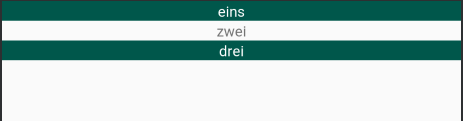
\includegraphics[scale=0.3]{img/linearlayout_1.png} 

\begin{lstlisting}[language=xml]
<LinearLayout 
    android:layout_width="match_parent"
    android:layout_height="match_parent"
    android:orientation="vertical">
    <TextView
        android:layout_width="match_parent"
        android:layout_weight="1"
        android:textAlignment="center"
        android:background="@color/colorPrimaryDark"
        android:textColor="#FFFFFF"
        android:text="eins"/>
    <TextView
        android:layout_width="match_parent"
        android:layout_weight="1"
        android:textAlignment="center"
        android:text="zwei"/>
    <TextView
        android:layout_width="match_parent"
        android:layout_weight="1"
        android:textAlignment="center"
        android:background="@color/colorPrimaryDark"
        android:textColor="#FFFFFF"
        android:text="drei"/>
</LinearLayout>
\end{lstlisting}

\includegraphics[scale=0.3]{img/linearlayout_2.png} 

\begin{lstlisting}[language=xml]
<LinearLayout 
 android:layout_width="match_parent"
 android:layout_height="match_parent"
 android:orientation="vertical">
 <TextView
    android:layout_width="match_parent"
    android:layout_height="wrap_content"
    android:layout_weight="0"
    android:textAlignment="center"
    android:background="@color/colorPrimaryDark"
    android:textColor="#FFFFFF"
    android:text="eins"/>
 <TextView
    android:layout_width="match_parent"
    android:layout_height="wrap_content"
    android:layout_weight="1"
    android:textAlignment="center"
    android:text="zwei"/>
 <TextView
    android:layout_width="match_parent"
    android:layout_height="wrap_content"
    android:layout_weight="0"
    android:textAlignment="center"
    android:background="@color/colorPrimaryDark"
    android:textColor="#FFFFFF"
    android:text="drei"/>
</LinearLayout>
\end{lstlisting}
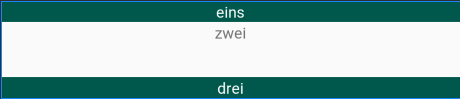
\includegraphics[scale=0.3]{img/linearlayout_3.png} 

\paragraph{Relative Layout}
\begin{lstlisting}[language=xml]
<RelativeLayout
 android:layout_width="match_parent"
 android:layout_height="match_parent">
 <TextView
    android:id="@+id/center"
    android:layout_width="wrap_content"
    android:layout_height="wrap_content"
    android:layout_centerInParent="true"
    android:text="Center"/>
 <TextView
    android:layout_width="wrap_content"
    android:layout_height="wrap_content"
    android:layout_toLeftOf="@id/center"
    android:layout_alignBottom="@id/center"
    android:text="2"/>
 <TextView
    android:layout_width="wrap_content"
    android:layout_height="wrap_content"
    android:layout_toRightOf="@id/center"
    android:layout_alignBottom="@id/center"
    android:text="3"/>
 <TextView
    android:layout_width="wrap_content"
    android:layout_height="wrap_content"
    android:layout_above="@id/center"
    android:layout_alignLeft="@id/center"
    android:text="1"/>
 <TextView
    android:layout_width="wrap_content"
    android:layout_height="wrap_content"
    android:layout_below="@id/center"
    android:layout_alignLeft="@id/center"
    android:text="4"/>
</RelativeLayout>
\end{lstlisting}
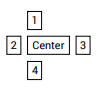
\includegraphics[scale=0.7]{relativelayout.png} \\
\textbf{Beispiele verstehen:} \\
Linke Kante ausrichten auf Linke Kante von ID-Element: \code{android:layout\_alignLeft} \\
Linke Kante ausrichten auf Rechte Kante von ID-Element: \code{android:layout\_toRightOf}\\
Unten/Oben ausrichten: \code{android:layout\_above | android:layout\_below}\\
Ausrichten am Parent: \code{android:layout\_centerInParent="true" | android:layout\_alignParentBottom="true"} etc. \\
\code{android:layout\_alignBaseline} um Text auf gleiche Höhe zu bringen (ohne Margin)
\paragraph{Weitere Layouts}
\begin{itemize}
  \item Frame Layout: Kinder übereinander anordnen (Linien bei einer Kamera App). In Activity Klasse mit \code{setContentView(R.layout.activity\_main)}
  \item FlexboxLayout: CSS Flexbox
  \item ConstraintLayout, mit RelativeLayout verwandt (war in Android Studio immer Standard ab irgendeiner Version)
  \item WebView um HTML anzuzeigen: JavaScript kann aktiviert werden, und Java-Objekte können mit JS angesprochen werden
\end{itemize}

\subsection{View setzen und GUI-Objekt finden finden}
\begin{lstlisting}[language=java]
//View Setzen
setContentView(R.layout.activity_main);
//View/Elemente finden
Button button = (Button) findViewById(R.id.button)
\end{lstlisting}
findViewById innerhalb einer Activity sucht im aktuellen Layout (wahrscheinlich dasjenige von \code{setContentView}). Rückgabe ist immer die Oberklasse \code{View},  das Resultat muss also noch gecastet werden.

Hat man allerdings ein Fragment oder z.B. ein Listenelement, so muss man die Parent-View vorher gespeichert haben (z.B. die Rückgabe des \code{LayoutInflater}), und dann auf dieser die gewünschte View finden. 

\subsection{Widgets}
Widgets ist ein Sammelbegriff für alle fix-fertigen Komponenten für User-Interfaces (Buttons, Images, Checkboxes etc.)

\paragraph{Button}
\begin{lstlisting}[language=xml]
<Button
    android:layout_width="wrap_content"
    android:layout_height="wrap_content"
    android:text="Alarm"
    android:id="@+id/alarmButton" />
\end{lstlisting}
Bei \code{<ImageButton/>} kann das Bild mit \code{android:src="..."} geladen werden.
\paragraph{Eingabefelder}
\begin{lstlisting}[language=xml]
<EditText
android:id="@+id/phone"
android:layout_width="match_parent"
android:layout_height="wrap_content"
android:inputType="phone|textCapSentences|textAutoCorrect" />
\end{lstlisting}
\paragraph{Referenzen und ID}
\begin{lstlisting}[language=java]
// ID setzen
android:id="@+id/id_name
// ID referenzieren 
android:layout_below="@id/id_name"
\end{lstlisting}
Die Klasse R enthält alle IDs und Ressourcen( Layoutdateien, drawable[Bilder], menu[Menüs], mipmap[Launcher Icon der App], values[strings, etc.]) als Konstanten. 
\paragraph{Ressourcen} Konstanten in \code{dimens.xml} werden für Grössen in den Layouts benutzt.
Die Ordnernamen müssen in Java-Namen umgewandelt werden können, dürfen also z.B. kein \code{-} enthalten. Gleiches gilt auch für  \code{strings.xml}. Zugriff mit  \code{getString(R.string.app\_name);} 

\begin{lstlisting}[language=xml]
<!-- Layout -->
<RelativeLayout xmlns:android="..." xmlns:tools="..."
  android:layout_width="match_parent"
  android:layout_height="match_parent"
  android:paddingLeft="@dimen/activity_horizontal_margin"
  android:paddingRight="@dimen/activity_horizontal_margin"
  android:paddingTop="@dimen/activity_vertical_margin"
  android:paddingBottom="@dimen/activity_vertical_margin"
  tools:context=".MainActivity">
<!-- dimens.xml -->
  <!-- Default screen margins, per the Android Design guidelines. -->
  <dimen name="activity_horizontal_margin">16dp</dimen>
  <dimen name="activity_vertical_margin">16dp</dimen>
</resources>
\end{lstlisting}
Grössenangeben von Views erfolgen in density-indepentent Pixels (dp oder dip). Bei Schriften verwendet man scale-independent Pixels (sp).
\paragraph{Events und Event Handling}\label{grundlagen:eventhandling} Das Android-Framework hat einen sogenannten Event-Loop (Looper). Dieser wartet bis ein Ereignis passiert und verarbeitet dieses dann. \textbf{Nur der Main-Thread darf das GUI verändern.} \\
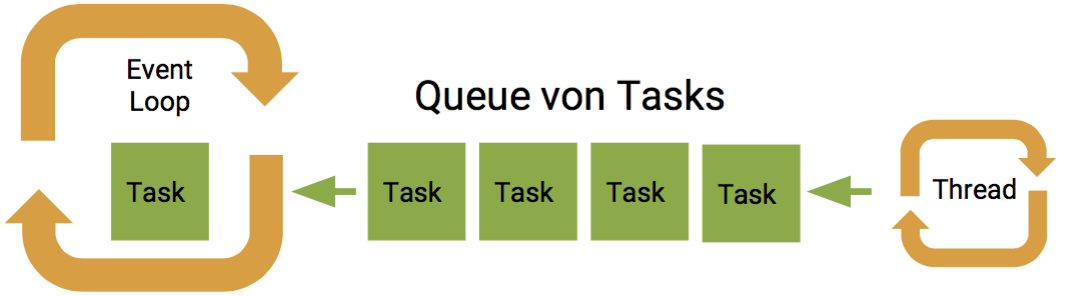
\includegraphics[scale=0.25]{EventLoops.png} \\

\paragraph{Event Listener}
Fast alle Listener können mit \code{set[EventName]Listener} registriert werden.
\begin{itemize}
    \item OnTouchListener: Touch Events
    \item OnClickListener: Wenn View angegklickt wird
    \item OnLongClickListener: touch and hold einer View
    \item OnKeyListener: wenn Hardware Taste ausgelöst wird.
\end{itemize}
\begin{lstlisting}[language=java]
button.setOnClickListener(new View.OnClickListener() {
  @Override
  public void onClick(View v) {
    /* ... */
  }
});
//oder direkt mit einem Lambda:
button.setOnClickListener( v -> { /* ... */ }); 
\end{lstlisting}
Oder onClick Listener in XML deklariert
 \begin{lstlisting}[language=java]
 // im xml:
 android:onClick="onButtonClicked"
 // onButtonClicked im Java implementieren
 public void onButtonClicked(View view) { /*....*/}
 \end{lstlisting}

Ein Listener lässt sich auch bei mehreren Views registrieren.
\begin{lstlisting}[language=java]
public void onClick(View view) {
    if (view == btn1) { // Code für btn1
    } else if (view == btn2) { // Code für btn2
}}
\end{lstlisting}

\paragraph{TextWatcher}
\begin{itemize}
\item \code{beforeTextChanged}: Wird aufgerufen bevor der Text geändert wird
\item \code{onTextChanged}: Wird aufgerufen sobald der Text geändert hat
\item \code{afterTextChanged}: Nachdem der Text geändert wurde, kann man den Text noch anpassen (Loop-Gefahr)
\end{itemize}
\begin{lstlisting}[language=java]
editText.addTextChangedListener(new TextWatcher() {
  public void onTextChanged(CharSequence s, int start, int before, int count){ }
  public void beforeTextChanged(CharSequence s, int start, int count, int after){ }
  public void afterTextChanged(Editable s) { }
});
\end{lstlisting}
\textbf{Inputvalidierung:}
\begin{lstlisting}[language=java]
final EditText password = (EditText) findViewById(R.id.password);
password.addTextChangedListener(new TextWatcher() {
  @Override
  public void afterTextChanged(Editable s) {
    String pw = s.toString();
    if (s.length() < 8) {
    password.setError("Passwort muss mindestens 8 Zeichen lang sein.");
    }
  }
  ...
});
\end{lstlisting}
%\subsection{Android Testing mit JUnit}
%Es gibt mehrere Arten von Tests für eine Activity. Die \code{ActivityUnitTest} manipulieren das UI im Code, die \code{ActivityInstrumentationTestCase2} schickt Clicks und Events an das UI. Um eine App mit mehreren Activities zu testen, gibt es das Espresso Framework, sowie UI Automator um App-übergreifend zu testen.
%\begin{lstlisting}[language=java]
%public class MainActivityLayoutTest extends ActivityUnitTestCase<MainActivity> {
%  public MainActivityLayoutTest() {
%    super(MainActivity.class);
%  }
%  @Override
%  protected void setUp() throws Exception {
%    super.setUp();
%    ContextThemeWrapper context = new
%      ContextThemeWrapper(getInstrumentation().getTargetContext(), R.style.AppTheme);
%    setActivityContext(context);
%    startActivity(
%      new Intent(getInstrumentation().getTargetContext(), MainActivity.class),null,null);
%}
%\end{lstlisting}
%Funktionale Tests (ActivityInstrumentationTestCase2) testen eine Activity im echten Systemkontext. Der Test löst Events aus und prüft, ob diese zum erwünschten Resultat führen. Dazu gehören: 
%\begin{itemize}
%\item Ändert sich das UI wie erwartet
%\item Überprüfen von Inputvalidierung
%\item Werden Lifecycle Events korrekt behandelt
%\end{itemize}
%\begin{lstlisting}[language=java]
%public class MainActivityInteractionTest extends ActivityInstrumentationTestCase2<MainActivity> {
%  public MainActivityInteractionTest() { super(MainActivity.class); }
%  public void testSayHi() {
%    MainActivity activity = getActivity();
%    final EditText editText = (EditText) activity.findViewById(R.id.editText);
%    getInstrumentation().runOnMainSync(new Runnable() {
%      @Override
%      public void run() {
%        editText.requestFocus();
%      }
%    });
%    getInstrumentation().waitForIdleSync();
%    getInstrumentation().sendStringSync("Hello");
%    getInstrumentation().waitForIdleSync();
%    Button button = (Button) activity.findViewById(R.id.button);
%    TouchUtils.clickView(this, button);
%...
%\end{lstlisting}

\section{Layout & Control Erweitert}
\subsection{Benutzerführung}
Die höchste Klasse jeder XAML App ist die \code{System.Windows.Application}. Beinhaltet:
    \begin{description}
        \item[Current] Property (Singelton) bietet statischen Zugriff auf das Application Objekt
        \item[MainWindow] das Zugriff auf das Hauptfenster bietet
        \item[ShutdownMode] welche das Verhalten beim Programmende definiert
    \end{description}

\paragraph{Current} Das Application Objekt ist als Singelton implentieret. Um es innerhalb der App zu verwenden, muss es oft gecastet werden.
\begin{lstlisting}
public App MyApp => Application.Current as App;
\end{lstlisting}
\paragraph{ShutdownMode} Der ShutdownMode definiert das Verhalten der App beim beenden, davon gibt es 3.
\begin{itemize}
\item \code{OnLastWindowClose}: Dies ist das Standardverhalten, die App beendet sich, sobald das letzte Fenster geschlossen wurde
\item \code{OnMainWindowClose}: Die App wird beendet sobald das Hauptfenster geschlossen wird
\item \code{OnExplicitShutdown}: Die App wird erst beendet, wenn die \code{Shutdown()} Methode aufgerufen wurde.
\end{itemize}
\paragraph{StartupUri} Dies ist der Name der UI Ressource, die beim Start angezeigt werden soll, es ist normalerweise ein \verb+Window+

\paragraph{Startup}

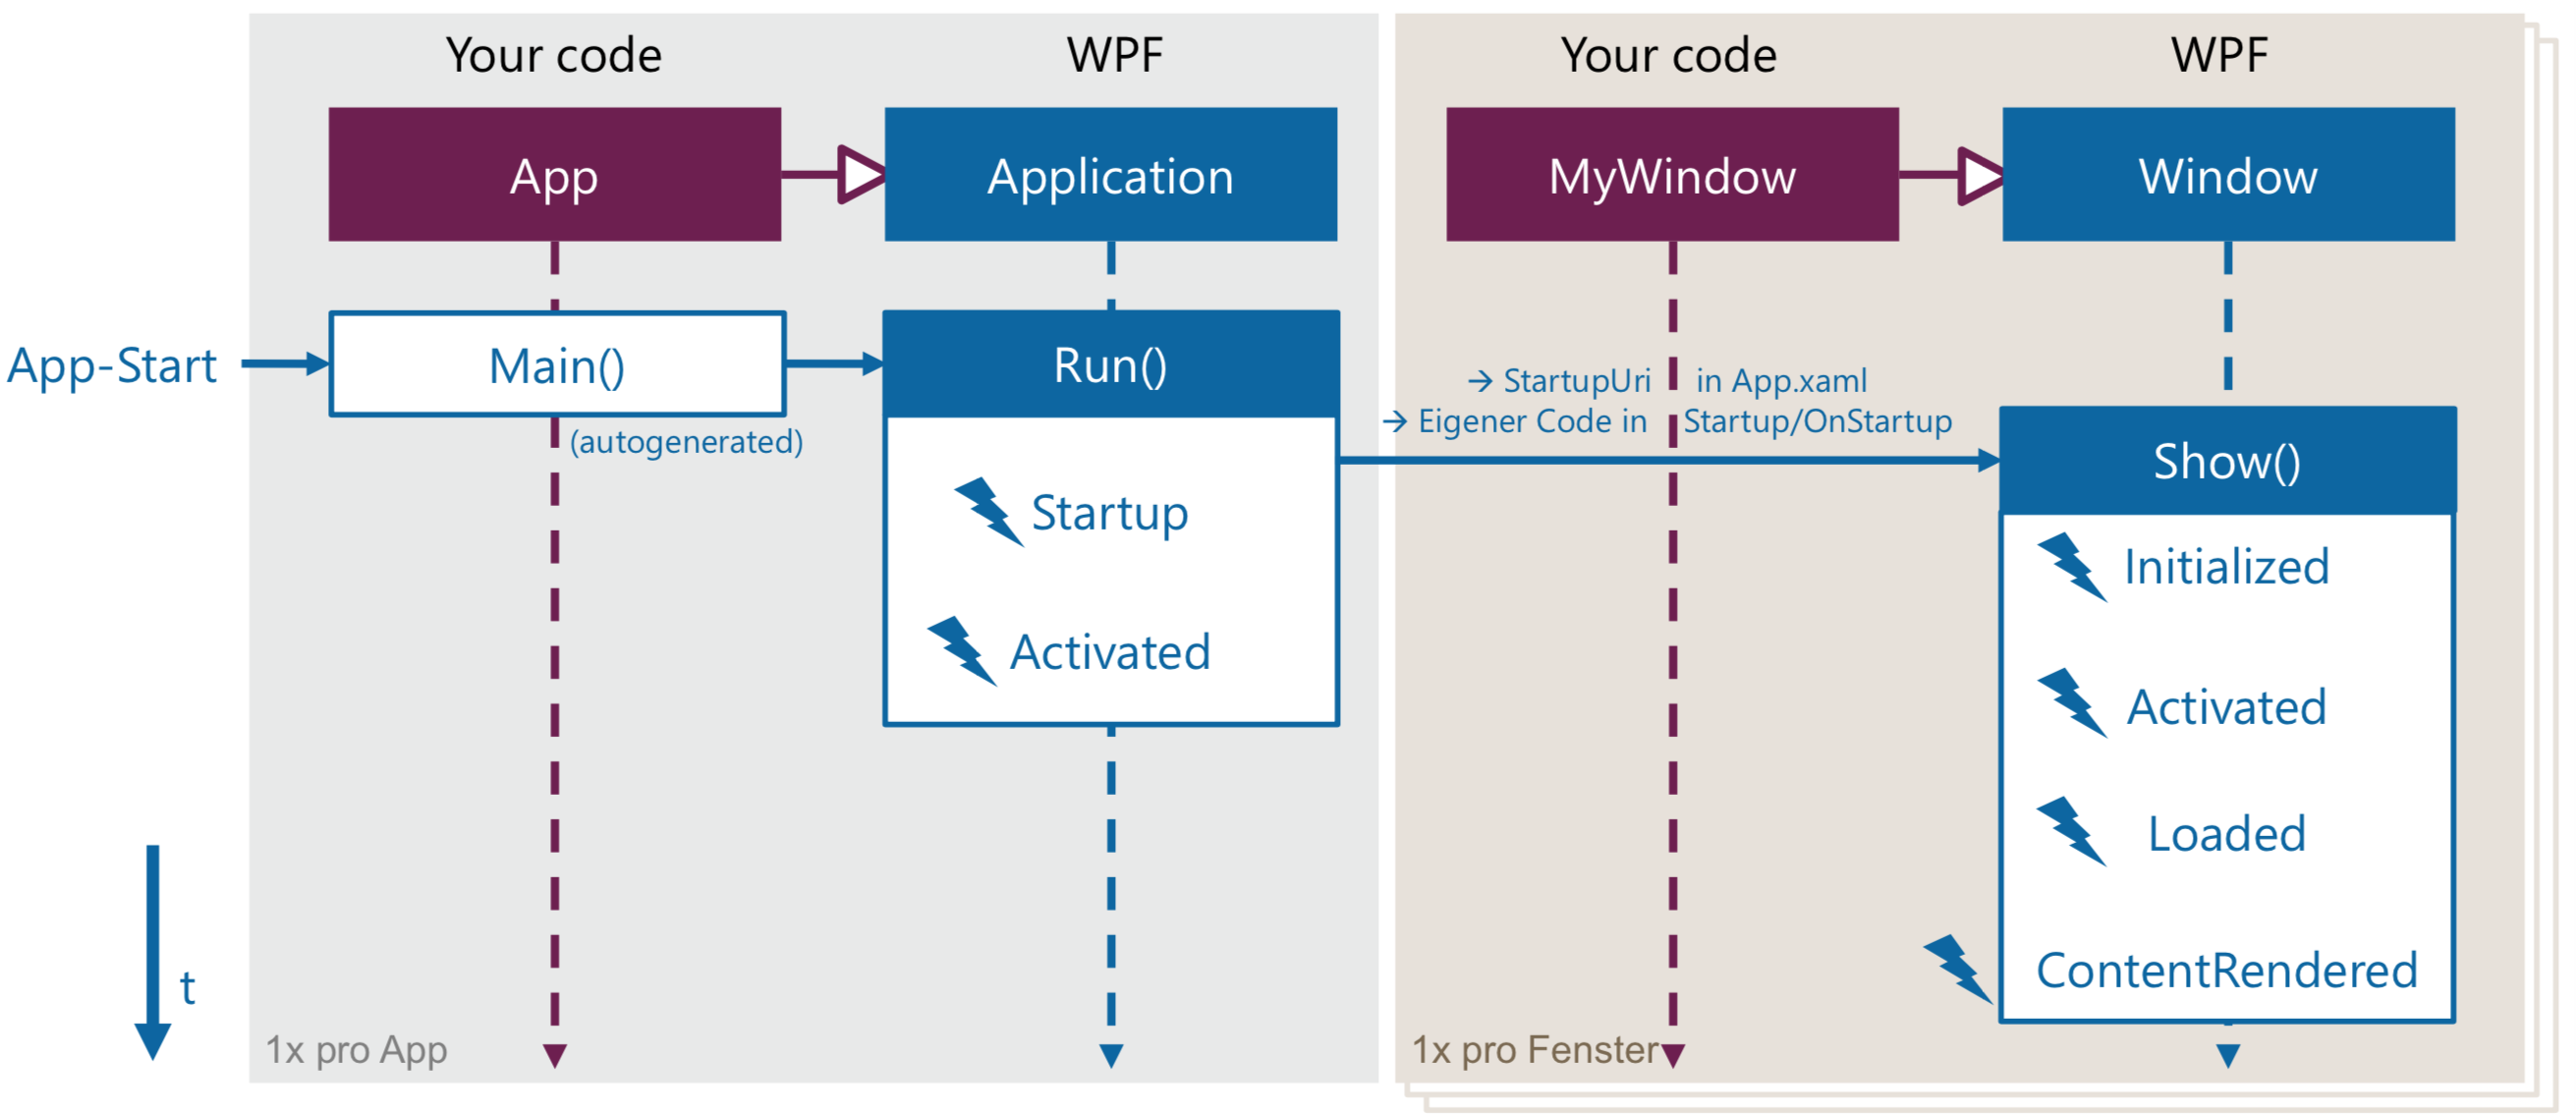
\includegraphics[scale=0.13]{startup.png}

\paragraph{Windows} Das \code{Windows} Property ist eine Liste aller instanziierter Fenster (Window-Objekte) innerhalb der App.
\paragraph{Application-Klasse Methoden} Die \verb+LoadComponent+ Methode lädt eine XAML-Ressource. Der Rückgabetyp muss in den korrekten Typ gecastet werden.
\begin{lstlisting}
public static object LoadComponent(Uri uri)
\end{lstlisting}
Die \verb+FindResouce+ Methode, sucht eine Ressource mit dem angegeben Namen. Es durchsucht App-Ressourcen und System-Ressourcen. Der Rückgabetyp muss ebenfalls in den korrekten Typ gecastet werden.
\begin{lstlisting}
public object FindResource(object resourceKey)
\end{lstlisting}
Die \verb+Shutdown+ Methode beendet die App und gibt optional einen mitgegebenen Exit Code ans System zurück.
\begin{lstlisting}
public void Shutdown([int exitCode])
\end{lstlisting}
\paragraph{Application-Klasse Events}
\begin{itemize}
\item \verb+Activated+: Die App wurde aktivitert (in den Vordergrund geholt)
\item \verb+Deactivated+: Die App wurde deaktiviert
\item \verb+DispatcherUnhandledException+: Eine nicht gefangene Exception ist aufgetreten
\item \verb+Exit+: Die App wird gleich beendet
\item \verb+FragmentNavitation+: Es wurde zu einem bestimmten \verb+NavigationWindow+/\verb+Frame+ navigiert
\item \verb+LoadCompleted+: Aktuelles \verb+NavigationWindow+/\verb+Frame+ wurde vollständig geladen
\item \verb+Navigated+: Aktuelles \verb+NavigationWindow+/\verb+Frame+ wurde gefunden
\item \verb+Navigating+: Navigation zu einem \verb+NavigationWindow+/\verb+Frame+  wurde angefordert
\item \verb+NavigationFailed+: Navigation zu einem \verb+NavigationWindow+/\verb+Frame+ ist fehlgeschlagen
\item \verb+NavigationProgress+: Statusinformation zum Downloadstatus bei Internet-Ressourcen
\item \verb+NavigationStopped+: Ladevorgang des Inhalts der \verb+NavigationWindow+/\verb+Frame+ wurde gestoppt
\item \verb+SessionEnding+: Windows Session wird beendet
\item \verb+Startup+: Die App startet gerade
\end{itemize}


\paragraph{SplashScreen} 
\begin{lstlisting}
private void App_OnStartup(object sender, StartupEventArgs e)
{
    var screen = new SplashScreen("media/splash.png");
    screen.Show(true);
}
\end{lstlisting}
\begin{lstlisting}
//App.xaml.cs
private void App_OnStartup(object sender, StartupEventArgs e)
{
    var screen = new SplashScreen("media/splash.png");
    screen.Show(true); // in den Folien steht false
    Thread.Sleep(2000);
    screen.Close(TimeSPan.FromMilliseconds(500));
}
\end{lstlisting}


\subsection{Window Klasse}
Die \verb+Window+ Klasse beschreibt ein Fenster. Sie ist abgeleitet von \verb+ContentControl+ und erlaubt genau 1 Child Element (\verb+LayoutContainer+).
\begin{itemize}
\item \verb+Icon+: Dieses Property beinhaltet eine ICO-Datei, die als Fenster Icon verwendet wird (Ausführbaren Datei und Fensterttitel)
\item \verb+ShowInTaskBar+: Ein Property das angibt, ob das Fenster in der Taskleite angezeigt wird
\item \verb+Topmost+: Zeigt Fenster über allen andern Fenstern der Anwendung an
\item \verb+SizeToContent+: Legt fest, ob die Grösse eines Fensters automatisch an die Grösse des Inhalts angepasst wird.
    \subitem \verb+Manual+: Fenstergrösse anhand Width/Height Angabe(Standart)
    \subitem \verb+Height+: Höhe wird automatisch anhand des Inhalts festgelegt
    \subitem \verb+Width+: Breite wird automatisch anhand des Inhalts festgelegt
    \subitem \verb+WidthAndHeight+: Breite und Höhe werden automatisch anhand des Inhalts festgelegt
\item \verb+ResizeMode+: Gibt an, wie sich die Fenstergrösse ändern darf. Je nach Einstellung werden zusätzlich die Schaltflächen Minimieren/Maximieren im Fenstertitel angezeigt
    \subitem \verb+NoResize+: Fenstergrösse nicht änderbar
    \subitem \verb+CanMinimize+: Fenster kann minimiert und wiederhergestellt werden
    \subitem \verb+CanResize+: Fenstergrösse kann frei verändert werden (Standard)
    \subitem \verb+CanResizeWithGrip+: Wie \verb+CanResize+ aber mit zusätzlichem Resize Grip unten rechts im Fenster
\item \verb+WindowsStartupLocation+: Legt die Postition beim Start fest
    \subitem \verb+CenterOwner+: Fenster wird in Mitte des aufrufenden angezeigt
    \subitem \verb+CenterScreen+: Fenster wird in der Mitte des Bildschirm angezeigt
    \subitem \verb+Manual+: Position wird durch Left/Top Angabe bestimmt (Standart)
\item \verb+WindowState+: Beschreibt die Fensterzustände (Normal, Minimized, Maximized)
\item \verb+WindowStyle+: Gibt den Rahmentyp des Fensters an:
    \subitem \verb+None+: Nur das Client Area ist sichtbar
    \subitem \verb+SingleBorderWindow+: Fenster mit einfachem (dünnem) Rahmen
    \subitem \verb+ThreeDBorderWindow+: Fenster mit 3D Rahmen
    \subitem \verb+ToolWindow+: Verankertes Tool-Fenster
\end{itemize}
\paragraph{Window-Klasse Methoden}
\begin{itemize}
\item \verb+Activate+: Fenster aktivieren
\item \verb+Close+: Fenster schliessen
\item \verb+DragMove+: Ermöglich das Verschieben des Fensters, falls die linke Maustaste gedrückt ist
\item \verb+GetWindow+: Statische Methode, ruft das Root-Window Objekt zum Control ab (DI)
\item \verb+Hide+: Macht das Fenster unsichtbar
\item \verb+Show+: Zeigt das Fenster an
\item \verb+ShowDialog+: Zeigt das Fenster an und blockiert, bis das Fenster geschlossen wird
\end{itemize}
\paragraph{Window-Klasse Events}
\begin{itemize}
\item \verb+Activated+: Fenster wurde aktiviert
\item \verb+Closed+: Fenster wurde geschlossen
\item \verb+Closing+: Fenster wird gleich geschlossen
\item \verb+ContentRendered+: Fensterinhalt wurde gezeichnet
\item \verb+Deactivated+: Fenster wurde deaktiviert
\item \verb+LocationChanged+: Position des Fensters wurde geändert
\item \verb+StateChanged+: WindowState hat geändert
\end{itemize}
\subsection{Mehrere Fenster}
In WPF ist es möglich mehrere Fenster zu definieren. Diese können zB mit einem ButtonClick angezeigt werden
\begin{description}
\item[.Show()-Methode] zeigt ein Fenster an (Mehrfensterbetrieb) (bei Android nicht möglich)
\item[.ShowDialog()-Methode] zeigt blockierend eine neues Fenster an (siehe nächste subsection)
\end{description}

\subsection{Dialogfenster} 
\begin{itemize}
    \item Dialogfenster dienen zum Abruf von Daten und sind meist Modal (blockierend).
    \item Ein Dialogfenster wird mit der Methode \verb+ShowDialog+ angezeigt. 
    \item Wird Property \code{DialogResult} gesetzt, wird das Dialogfenster automatisch geschlossen
\end{itemize}

\begin{lstlisting}[language=xml]
<Button Content="Cancel" IsCancel="true" />
<Button Name="OkButton" Content="OK" IsDefault="true" Click="OkButton_OnClick" />
\end{lstlisting}
Das \verb+IsCancel+ Property schliesst bei \verb+true+ das Dialogfenster automatisch (kein Event-Handling).
\begin{lstlisting}
private void OkButton_OnClick(object sender, RoutedEventargs e)
{
    SelectedCustomer = "MaxMuster";
    // trigger dialog close as side effect
    DialogResult = true; 
}
\end{lstlisting}
\begin{lstlisting}[language=sharpc]
private void OkButton_OnClick(object sender, RoutedEventargs e)
{
    var win = new DialogWindow();
    // blockiert bis Dialogfenster geschlossen
    if (win..Showdialog() != true)
    {
        return;
    }
    // Nun allfällige eingegeben Daten abrufen:
    var chosenCustomer = win.SelectedCustomer;
    ...
}
\end{lstlisting}

% \paragraph{Fenster mit Spezialformen} Die Fensterrahmen können mittels Clipping verändert werden. Das setzt jedoch folgende Fenstereigenschaften voraus:
% \begin{itemize}
% \item \verb+AllowsTransparency=true+
% \item \verb+WindowStyle=none+
% \item \verb+ResizeMode=NoResize+
% \end{itemize}
% Man kann die Form in \verb+Window.Clip+ mittels einem Geometry-Element festlegen
% \begin{lstlisting}[language=xml]
% <!-- Rechteck mit abgerundeten Raendern -->
% <Window.Clip>
%     <RectangleGeometry RadiusX="8" RadiusY="8" Rect="0,0,800,600" />
% </Window.Clip>
% \end{lstlisting}


% \subsection{Menu}
% Die Menüs sind herkömmliche Windows-Menüs und werden üblicherweise am oberen Fensterrand angedockt. Mit dem Property \verb+IsMainMenu=true+ kann man das Menü standartmässig als Hauptmenü definieren.
% \paragraph{MenuItem} MenuItems sind beliebig verschachtelbar. Sie haben ein \verb+Header+ als anzuzeigenden Texts (Underscore = Accelerator-Key), \verb+IsCheckable+ definiert, ob der Eintrag ein Zustand ist (mit \verb+IsChecked+ kann Zustand gesetzt bzw. geprüft werden). Das \verb+InputGestureText+ Property definiert, definiert einen Text, der im MenuItem rechtsbündig angezeigt wird (Shortcuts wie Ctrl+V), um zu Funktionieren müssen diese noch behandelt werden, beispielsweise mit Commands.
% \begin{lstlisting}[language=xml]
% <Menu DockPanel.Dock="Top">
%     <MenuItem Header="_File">
%         <MenuItem Header="_Recent">
%             <MenuItem Header="Secret.txt" />
%             <MenuItem Header="TopSecret.txt" />
%         </MenuItem>
%         <Separator />
%         <MenuItem Header="E_xit" InputGestureText="CTRL + Q" />
%     </MenuItem>
%     <MenuItem Header="_Edit">
%         <MenuItem Header="_Cut" InputGestureText="CTRL + X" />
%         <MenuItem Header="C_opy" InputGestureText="CTRL + C" />
%         <MenuItem Header="_Paste" InputGestureText="CTRL + V" />
%         <Separator />
%         <MenuItem Header="_Settings">
%             <MenuItem Header="_Always On Top" IsChecked="True"></MenuItem>
%             <MenuItem Header="_Modern UI" IsChecked="false"></MenuItem>
%         </MenuItem>
%     </MenuItem>
% </Menu>
% \end{lstlisting}
% \paragraph{Kontextmenus} Das \verb+ContextMenu+ stellt ein kontextspezifisches Menü zur verfügung. Es funktioniert wie das Menü und kann direkt mit der Property-Syntax für ein Control erstellt werden.
% \begin{lstlisting}[language=xml]
% <Button.ContextMenu>
%     <ContextMenu>
%         <MenuItem Header="Hilfe" />
%         <MenuItem Header="Fehler melden" />
%     </ContextMenu>
% </Button.ContextMenu>
% \end{lstlisting}
% \paragraph{StatusBar} Die Statusbar dient zur Anzeige von zusätzlichen Informationen (meist am unteren Fensterrand). Es ist ein Container, ähnlich wie beim DockPanel, dabei füllt das letzte Element die ganze restliche Breite.
% \begin{lstlisting}[language=xml]
% <StatusBar DockPanel.Dock="Bottom">
%     <StatusBarItem Width="150">Press CTRL + Q to quit</StatusBarItem>
%     <Separator />
%     <StatusBarItem>Ready</StatusBarItem>
% </StatusBar>
% \end{lstlisting}
% Für Kontextbezogene Statusinformationen können \verb+StatusBarItem+ Elemente benannt werden und dann programmatisch darauf zugegriffen werden, oder man arbeitet mit Databinding.
% \paragraph{Toolbar} kann entweder ein \verb+ToolBarTray+ sein, der als Container für Toolbars dient, oder ein \verb+Toolbar+ der als Container für Toolbar-Buttons und sonstige Toolbar-Controls dient. Die ToolBarTray ermöglicht das Verschieben und Umgruppieren der Toolbars und ist typischerweise angedockt. \\
% 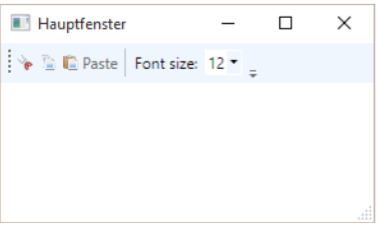
\includegraphics[scale=0.40]{Toolbar.png}
% \begin{lstlisting}[language=xml]
% <ToolBarTray DockPanel.Dock="Top">
%     <ToolBar>
%         <Button Command="Cut" ToolTip="...">
%             <Image Source="/media/clip_cut.png" Width="12" Height="12" />
%         </Button>
%     <Button Command="Copy" ToolTip="Copy selection to Windows Clipboard.">
%         <Image Source="/media/clip_copy.png" Width="12" Height="12" />
%     </Button>
%     <Button Command="Paste" ToolTip="Paste from Windows Clipboard.">
%         <StackPanel Orientation="Horizontal">
%             <Image Source="/media/clip_paste.png" Width="12" Height="12" />
%             <TextBlock Margin="3,0,0,0">Paste</TextBlock>
%         </StackPanel>
%     </Button>
%     <Separator />
%     <Label>Font size:</Label>
%     <ComboBox>
%         <ComboBoxItem>10</ComboBoxItem>
%         <ComboBoxItem IsSelected="True">12</ComboBoxItem>
%         <ComboBoxItem>14</ComboBoxItem>
%         <ComboBoxItem>16</ComboBoxItem>
%     </ComboBox>
%     </ToolBar>
% </ToolBarTray>
% \end{lstlisting}
% \paragraph{Ribbon} Das Ribbon ist seit Office 2007 bekannt und ist seither immer stärker verbreitet. 
% \begin{lstlisting}[language=xml]
% <Ribbon Name="Ribbon">
%     <Ribbon.ApplicationMenu>
%         <RibbonApplicationMenu SmallImageSource="media/home.png">
%             <RibbonApplicationMenuItem Header="Hello _Ribbon"
%                 Name="MenuItem1"
%                 ImageSource="media/home.png"/>
%         </RibbonApplicationMenu>
%     </Ribbon.ApplicationMenu>
%     <RibbonTab x:Name="HomeTab" Header="Start">
%         <RibbonGroup x:Name="Clipboard" Header="Clipboard">
%             <RibbonButton x:Name="Button1" Label="Paste"
%                 LargeImageSource="media/clip_paste.png" />
%             <RibbonButton x:Name="Button2" Label="Cut"
%                 SmallImageSource="media/clip_cut.png" />
%             <RibbonButton x:Name="Button3" Label="Copy"
%                 SmallImageSource="media/clip_copy.png" />
%         </RibbonGroup>
%     </RibbonTab>
% </Ribbon>
% \end{lstlisting}
% 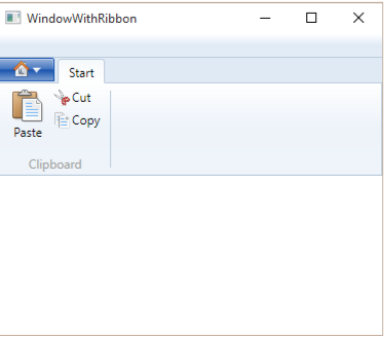
\includegraphics[scale=0.35]{Ribbon.png}
% \section{Commands} bieten eine Alternative zum Event. Commands müssen nicht abgefangen und behandelt werden, sie werden durch die Control selbst aufgerufen. Es ist eine standartisierte Ausführung eines Befehls und ermöglicht die Wiederverwendung derselben Aktion. Eine Command-Methode muss \verb+RoutedUICommand+ als Rückgabetyp haben und statisch sein.
% \begin{lstlisting}
% public static RoutedUICommand MyCutCommand = new RoutedUICommand(
%     "Ausschneiden",
%     "MyCut",
%     typeOf(WindowWithToolbar)
% );
% \end{lstlisting}
% Der \verb+RoutedUICommand+ nimmt auch noch einen 4. Paramter entgegen, in dem man \verb+InputGestures+ entweder einzeln oder als \verb+InputGestureCollection+ mitgeben kann.
% \begin{lstlisting}[language=xml]
% <MenuItem Header="_Cut" InputGestureText="CTRL + X" Command="local:WindowWithToolbar.MyCutCommand" />
% \end{lstlisting}
% Commands können auch an Event-Handler gebunden werden und Shortcuts definiert werden.
% \begin{lstlisting}[language=xml]
% <!-- Binding an Event -->
% <Window.CommandBindings>
%     <CommandBinding Command="local:WindowWithToolbar.MyCutCommand" Executed="MyCutCommand_Executed" />
% </Window.CommandBindings>
% <!-- Shortcut definieren -->
% <Window.InputBindings>
%     <KeyBinding Key="X" Modifiers="Control" Command="local:WindowWithToolbar.MyCutCommand" />
% </Window.InputBindings>
% \end{lstlisting}
% Im Code-Behind kann dann wie gewohnt ein Handler definiert werden.
% \begin{lstlisting}
% public void MyCutCommand_Executed(object sender, ExecutedRoutedEventArgs e){ ... }
% \end{lstlisting}
% \section{Automated UI Testing}
% 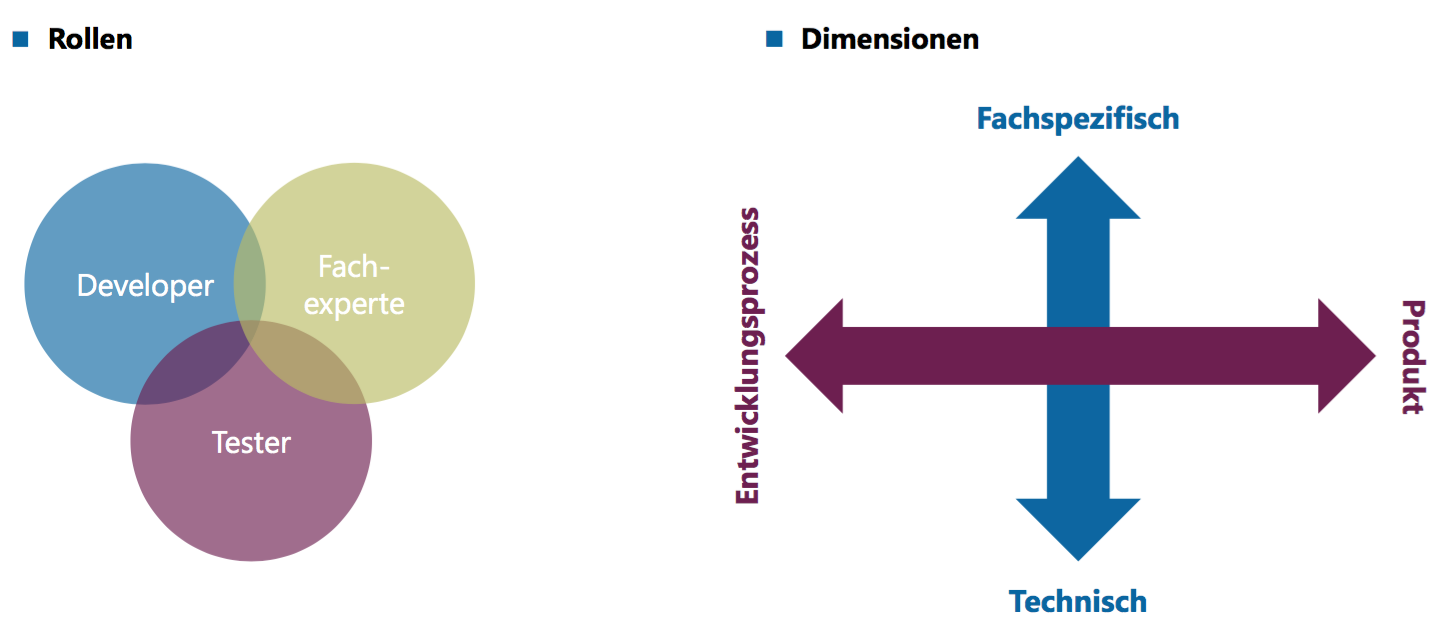
\includegraphics[scale=0.25]{Testing1.png}
% 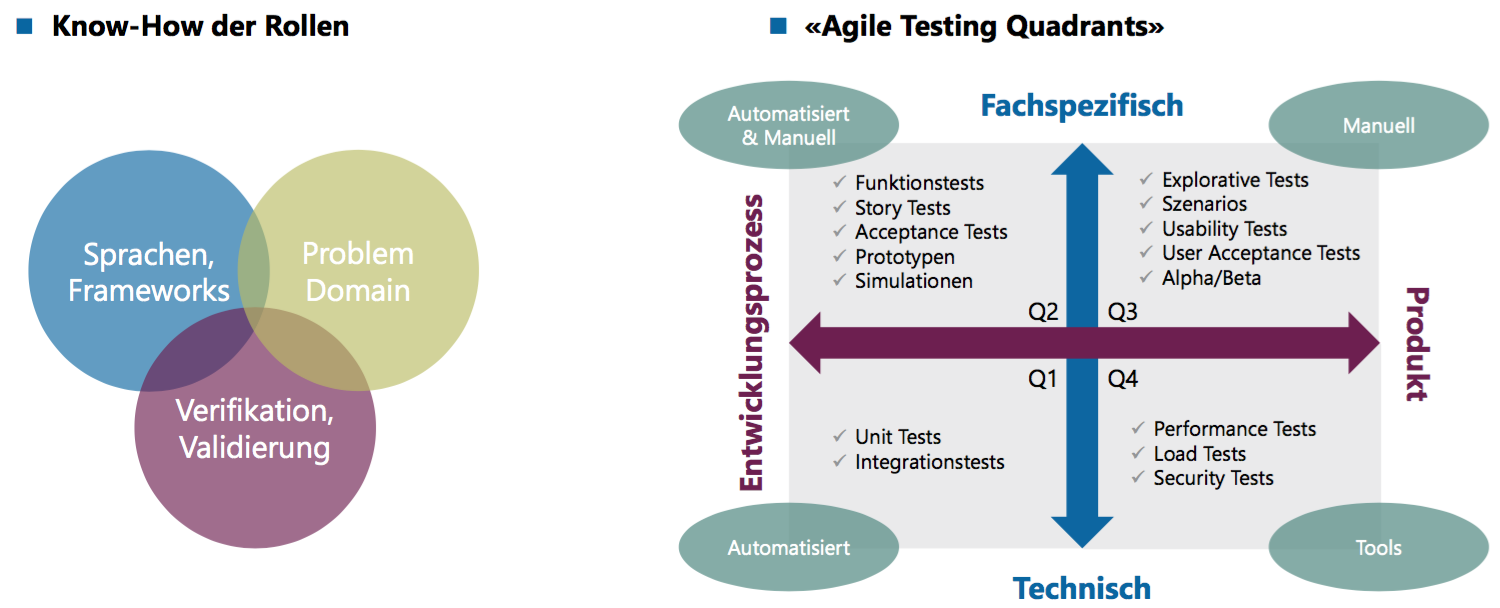
\includegraphics[scale=0.25]{Testing2.png}
% 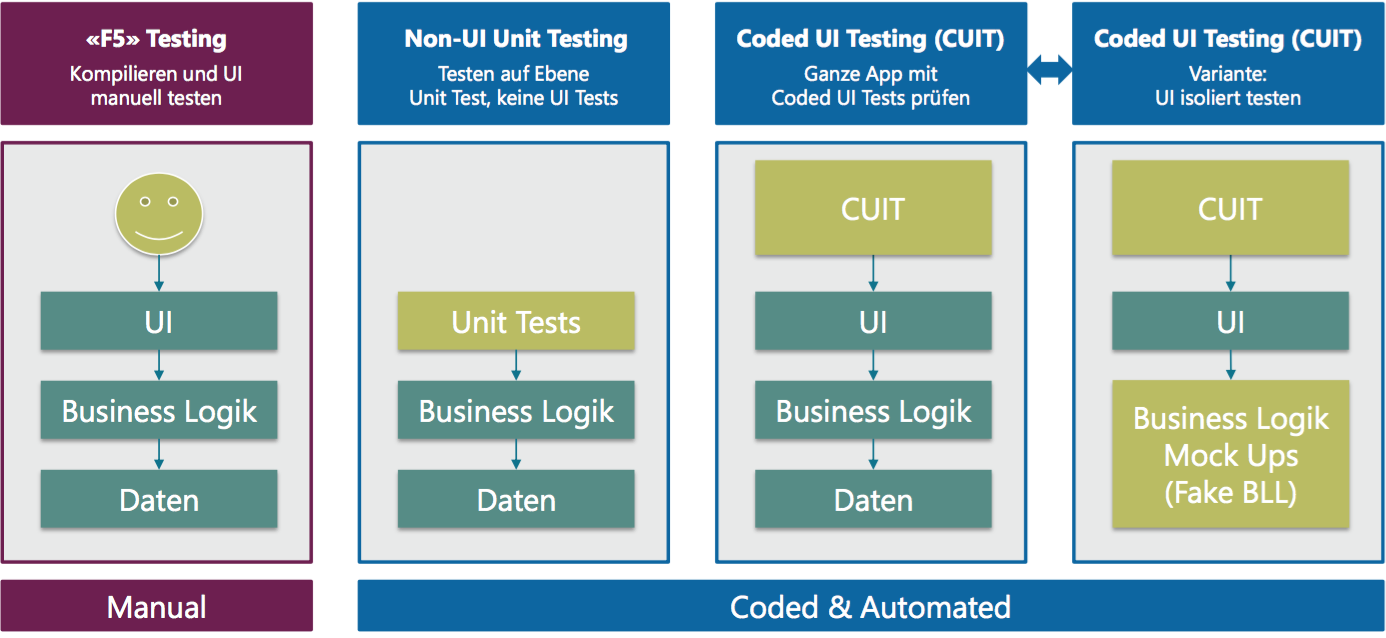
\includegraphics[scale=0.25]{Testing3.png} \\
% Es gibt 4 Varianten UIs zu testen. Das \textbf{Non-UI Unit Testing} Test auf Code Ebene (normale Unit-Tests) und führt keine UI-Tests durch. Das \textbf{Coded UI Testing (CUIT)} testet die ganze App mit Coded UI Tests. Diese Variante kann man auch mit isolierten UI Komponenten durchführen, welche dann aber Fake Komponenten benötigen (die 4. Variante ist das F5-Testing, der Benutzer testet die App gleich selbst).
% \subsection{TestStack}
% Der TestStack ist eine Sammlung von OpenSource Projekten um Tests in .NET Projekten zu automatisieren. Dazu gehört das \textbf{TestStack.White} Framework. Es ist ein CUIT-FW für WPF und basiert auf Microsofts UI Automation Framework. \\
% Als Vorbereitung muss man eine Testklasse erstellen.
% \begin{lstlisting}
% [TestClass]
% public class MyUiTest
% {
%     [TestMethod]
%     public void MyUiTestMethod(){ ... }
% }
% \end{lstlisting}
% Danach muss man das Verzeichnis mit der WPF App Assembly festlegen. Dies kann dann als Read-Only Property in der Testklasse hinzugefügt werden.
% \begin{lstlisting}
% // Directory in which tests are running
% public string BaseDir => Path.GetDirectoryName(Assembly.GetExecutingAssembly().Location);
% // System under test
% public string SutPath => Path.Combine(BaseDir, ${nameof(MenusAndCommands)}.exe);
% //$
% \end{lstlisting}
% Nun kann man die Tests entwickeln. \\
% Zuerst neues Application Objekt aus dem WPF App Assembly erstellen:
% \begin{lstlisting}
% var app = Application.Launch(SutPath);
% \end{lstlisting}
% Die Variable enthät ein UI-Automatisierungsobjekt des Typs \verb+TestStack.Whie.Application+.
% Danach kann man die Fenster abrufen:
% \begin{lstlisting}
% // Mit Fenstertitel abrufen
% var window = app.GetWindow("Hauptfenster", InitializeOption.NoCache);
% // Aus Liste der Fenster abrufen
% var window = app.GetWindows.First();
% // Anhand der ID(Name-Attribut) abrufen
% var window = app.getWindow(SearchCriteria.ByAutomationId"(Win1"), InitializeOption.NoCache);
% \end{lstlisting}
% Die Variable \verb+window+ enthäht nun ein UI-Automatisierungsobjekt des Typs \verb+TestStack.White.UIItems.WindoItems.Window+.\\
% Danach muss man die Controls abrufen:
% \begin{lstlisting}
% // Anhand Beschriftung abrufen
% var button = window.Get<Button>(SearchCriteria.ByText("Speichern"));
% // Anhand ID(Name-Attribut) abrufen
% var button window.Get<Button>("SaveButton");
% \end{lstlisting}
% Die Variable \verb+button+ enthält nun ein UI-Automatisierungsobjekt des Typs \verb+TestStack.White.UIItems.Button+.\\
% Schlussendlich können Aktionen ausgeführt werden:
% \begin{lstlisting}
% Assert.AreEqual("Speichern", button.Text);
% button.Click();
% Assert.AreEqual("Gespeichert!", button.Text);
% \end{lstlisting}
% \begin{lstlisting}
% var input = window.Get<TextBox>("NameInput");
% Assert.IsTrue(string.IsNullOrEmpty(input.Text));
% var newText = "You've been hacked!";
% input.Text = newText;
% Assert.AreEqual(newText, input.Text);
% \end{lstlisting}
% Schlussendlich muss die App noch mittels \verb+app.Close()+ beendet werden.\\
% Mit \verb+Desktop.CaptureScreenshot()+ erhält man ein Bitmap Objekt mit einem Bild des aktuellen Bildschirms.
% \begin{lstlisting}
% var screenshot = Desktop.CaptureScreenshot();
% var path = System.IO.Path.Combine(BaseDir, "screenshot.png");
% screenshot.Save(path, ImageFormant.Png);
% \end{lstlisting}


\section{GUI Design}
\paragraph{WPF Ressourcen}
Mit WPF Ressourcen kann man nützliche Objekte (Image, Brushes, Styles, Templates etc.) zentral definieren und wiederverwenden.


\paragraph{Physikalische Ressourcen} In den File Properties kann man eine Datei als WPF-Ressource deklarieren welche dann in die Binärdatei einkompiliert werden. Zugegriffen kann dann mittels Resource-Key (relativer Pfadname).
\begin{lstlisting}[language=xml]
<Image Source="Desert.jpg" />
\end{lstlisting}


\paragraph{Resource}
\begin{itemize}
    \item Beliebige Objekte in XAML können als Ressource definiert werden
    \item Wird mit dem Key-Attribut aus dem x-Namespace benannt
\end{itemize}
\begin{lstlisting}[language=xml]
<Application.Resources>
    <SolidColorBrush x:Key ="MyButtonBackground" Color="#EEEEEE" />
</Application.Resources>
\end{lstlisting}
Unter diesem Key sind Ressourcen dann auch ansprechbar
\begin{lstlisting}[language=xml]
<Button ...>
  <Button.Background>
    <StaticResource ResourceKey="MyBg" />
  </Button.Background>
</Button>

<Button Background="{StaticResource MyButtonBackground}" Content="Save" />
\end{lstlisting}


\paragraph{ResourceDictionary} 
\begin{itemize}
    \item Behälter um Ressourcen zu speichern
    \item Indexiert nach Ressourcen-Namen (\verb+x:Key+)
    \item In mehrere Elementen out-of-the-box verfügbar
    \begin{itemize}
        \item Application.Resources
        \item Window.Resources
        \item Button.Resources
        \item Label.Resources
    \end{itemize}
    \item Schont die Ressourcen (Mehrfachverwendung)
    \item Die Reihenfolge im XAML ist wichtig
\end{itemize}



\paragraph{FindResource} Mit der Methode \verb+FrameworkElement.FindResources+  können Zugriffe auf XAML Resourcen im Code-behind gemacht werden.
\begin{lstlisting}
var okText = (string)FindResource("OkText");
var bgBrush = FindResource("DarkBrush") as Brush;
\end{lstlisting}

\subsubsection{Zugriff}
\begin{enumerate}
    \item Key wird im Element und in allen Parent-Nodes gesucht.
    \item Key wird in Application.Resources gesucht.
    \item Key wird in System-Ressourcen gesucht.
\end{enumerate}

% \paragraph{System Ressources} Auf Ressourcen in Namespace \verb+System.Windows+ kann man mittels statischer Properties zugegriffen werden. Dazu gehören: \verb+SystemColors+, \verb+SystemFonts+ und \verb+SystemParamters+.
% \begin{lstlisting}[language=xml]
% StaticResource="{StaticResource[name]}"
% \end{lstlisting}
% Die Statische Bindung macht CompileTime Check und findet Fehler früh.
% \begin{lstlisting}[language=xml]
% DynamicResource="{DynamicResource[name]}"
% \end{lstlisting}
% Anstelle von \verb+[name]+ steht der Key der Ressource
% In der Dynamische Bindung wird ein RuntimeCheck gemacht und lässt dynamisch erzeugte und geladene Ressourcen zu. Beim Static Binding wird bei Objektkonstruktion ausgewertet, beim Dynamic Binding einmal pro Zugriff.

\paragraph{Static vs DynamicResource}
\begin{lstlisting}[language=xaml]
<Button ... Background="{StaticResource MyBg}" />
<Button ... Background="{DynamicResource MyBg}" />
\end{lstlisting}

\textbf{Static Resources}
\begin{itemize}
    \item Anstelle von \code{name} steht der Key der Ressouce
    \item Statische Bindung an Ressource $\Longrightarrow$ 1-malig beim Laden
    \item Compile Time Check $\Longrightarrow$ findet den Fehler früh 
\end{itemize}
\textbf{Dynamic Resources}
\begin{itemize}
    \item Anstelle von \code{name} steht der Key der Ressouce
    \item Dynamische Bindung (bei jedem Zugriff)
    \item Runtime Check $\Longrightarrow$ lässt dynamisch erzeuge Ressourcen zu
\end{itemize}


\paragraph{Eigene ResourceDictionaries}
\begin{itemize}
    \item Separates xaml-File
    \item In andere ResourceDictionaries einbindbar
    \item XML-Root-Node ist <ResourceDictionary>
\end{itemize}
\begin{lstlisting}[language=xml]
<ResourceDictionary xmlns="http://schemas.microsoft.com/winfx/2006/xaml/presentation" xmlns:x="http://schemas.microsoft.com/winfx/2006/xaml" xmlns:local="clr-namespace:Microsoft.FamilyShow"> 

  <!-- place your resources here --> 
  
</ResourceDictionary> 
\end{lstlisting}

Zum Einbinden muss ein \code{MergedDictionary} verwendet werden:
\begin{lstlisting}[language=xml]
<Application.Resources>
  <ResourceDictionary>
    <!– you can mix resources and merged dictionaries -->
    <SolidColorBrush x:Key ="MyButtonBackground" Color="#EEEEEE" />
   
    <ResourceDictionary.MergedDictionaries>
      <!– just list your external resource dictionaries, here --> 
      <!– (the order is important!) -->
      <ResourceDictionary Source="Colors.xaml"/>
      <ResourceDictionary Source="Brushes.xaml"/>
      </ResourceDictionary.MergedDictionaries>
    </ResourceDictionary>
</Application.Resources> 
\end{lstlisting}

\section{Externe Resources einbinden}
Für das Einbinden von externen Ressourcen, z.B Bilder, gibt es verschiedene Möglichkeiten.
\paragraph{Gleiche Assembly}
Einbinden einer Ressource von derselben Assembly:
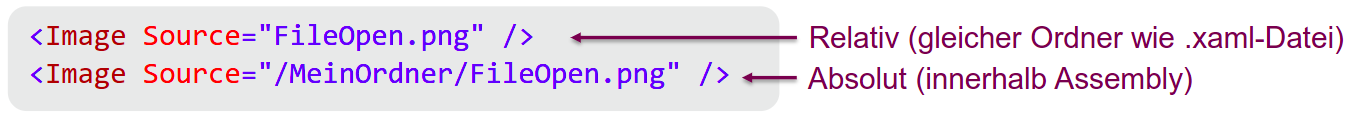
\includegraphics[scale=0.18]{img/resource-same-assembly.png}

\paragraph{Externe Assembly}
Einbinden einer Ressourcen von einer anderen Assembly:
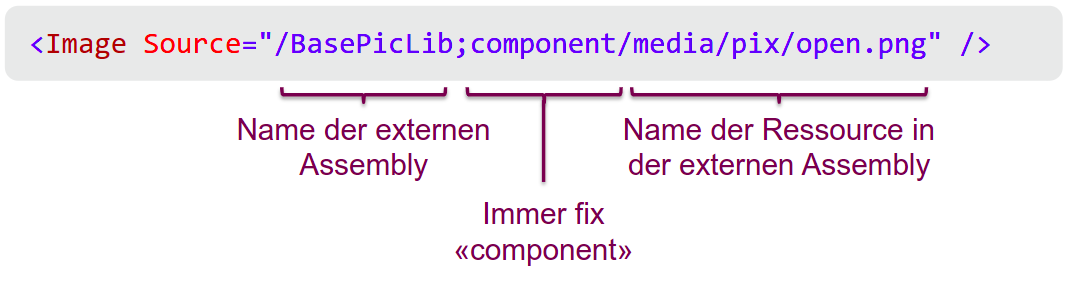
\includegraphics[scale=0.22]{img/ressource-other-assembly.png}

\paragraph{Absolute Angabe}
Sollte nicht verwendet werden, da bei jeder Umgebung anders (zu starke Bindung).

\paragraph{PackageURI}
Es wird ein PackageURI verwendet, welcher spezifiziert, 
\begin{lstlisting}[language=xml]
<!--Relativ zum aktuellen Ordner--!>
<Image Source="pack://siteOfOrigin:,,,/media/pix/open.png" />
<!--Relativ zur Assembly--!>
<Image Source="pack://application:,,,/media/pix/open.png" /> 
\end{lstlisting}

\paragraph{Zugriff aus statische Werte (z.B System Ressourcen)}
Es gibt verschiedene System-Ressourcen:
\begin{itemize}
    \item SystemColors - z.B SystemColors.WindowTextColor
    \item SystemFonts - z.B SystemFonts.MenuFontFamily
    \item SystemParameters - z.B SystemParameters.PrimaryScreenWidth
\end{itemize}
\begin{lstlisting}
<Button Background="{x:Static SystemColors.ControlBrush}" Content="Save" /> 
<TextBox FontFamily="{x:Static SystemFonts.MenuFontFamily}" > ... 
\end{lstlisting}

\section{Styles}
Das Aussehen sollte ausschliesslich über Styles und Templates definieren werden! 
\subsubsection{implizit (typspezifisch)}
\begin{itemize}
    \item \textbf{x:Key} wird weggelassen
    \item \code{TargetType="Button"} benutzen
    \item Klassenname (\code{Button.Foreground}) kann weggelassen werden
    \item Style gilt für alle Elemente wenn man den Key weglässt
\end{itemize}
\begin{lstlisting}[language=xml]
<!-- App.xaml -->
<Application x:Class="ModernUi.App"
             xmlns="http://schemas.microsoft.com/winfx/2006/xaml/presentation"
             xmlns:x="http://schemas.microsoft.com/winfx/2006/xaml"
             xmlns:local="clr-namespace:ModernUi"
             StartupUri="MainWindow.xaml">
    <Application.Resources>
        <ResourceDictionary Source="style.xaml"></ResourceDictionary>
    </Application.Resources>
</Application>
\end{lstlisting}
\begin{lstlisting}[language=xml]
<!-- Style.xaml -->
<Window.Resources>
    <!-- benannten Style als Basis benutzen -->
    <Style x:Key="DefaultButtonStyle" TargetType="Button">
      <Setter Property="BorderThickness" Value="1" />
      <Setter Property="BorderBrush" Value="Black" />
      <Setter Property="Background" Value="Transparent" />
      <Setter Property="Foreground" Value="Black" />
      <Setter Property="FontFamily" Value="Segoe UI" />
      <Setter Property="Margin" Value="2" />
      <Setter Property="Padding" Value="10 2 10 2" />
      <Setter Property="FontSize" Value="13" />
    </Style>
    
    <!-- Den obigen benannten Style erben und auf alle Buttons anwenden -->
    <Style TargetType="Button" BasedOn="{StaticResource DefaultButtonStyle}"> </Style>
    
    <!-- fuer den Help Button noch einen abgeleiteten Style definieren --> 
    <Style x:Key="MyHelpButtonStyle" TargetType="Button"
           BasedOn="{StaticResource DefaultButtonStyle}">
      <Setter Property="Foreground" Value="Gray" />
      <Setter Property="BorderBrush" Value="Gray" />
    </Style>
</Window.Resources>
\end{lstlisting}
\begin{lstlisting}[language=xml]
<!-- Window.xaml -->
<Button Style="{StaticResource DefaultButtonStyle}" Content="OK" />
\end{lstlisting}

\subsubsection{explizit}
Haben einen expliziten \textbf{x:key}
\begin{lstlisting}[language=xml]
<Style x:Key="MyButtonStyle">
    <Setter Property="Button.Foreground" Value="#000000" />
    <Setter Property="Button.Background" Value="#FFFFFF" />
    <!-- auch komplexes möglich -->
    <Setter Property="Button.Background">
        <Setter.Value>
            <LinearGradientBrush StartPoint="0,0" EndPoint="0,1">
                <GradientStop Offset="0" Color="#dddddd"></GradientStop>
                <GradientStop Offset="0.5" Color="#F0F0F0"></GradientStop>
                <GradientStop Offset="1" Color="#dddddd"></GradientStop>
            </LinearGradientBrush>
        </Setter.Value>
    </Setter>
</Style>
\end{lstlisting}
Verwenden mit:
\begin{lstlisting}[language=xml]
<Button Style="{StaticResource MyButtonStyle}" Content="Cancel" />
\end{lstlisting}



\subsubsection{Styles kombinieren}
\begin{itemize}
    \item Styles können abgeleitet werden
    \item Styles mit Inline Eigenschaften kombinierbar
\end{itemize}
\begin{lstlisting}[language=xml]
<Style x:Key="DangerButtonStyle" 
      TargetType="Button" 
      BasedOn="{StaticResource MyButtonStyle}"> 
  <Setter Property="Background" Value="Red" /> 
</Style> 
\end{lstlisting}

\subsection{Control Templates}
\begin{itemize}
    \item Legt die Inhaltsdarstellung eines Controls fest
    \item Für alle visuellen Control-Typen vorgegeben
    \item Jede Windows Version hat passendes Theme
    \item Legt Standard-Aussehen eines XAML Controls fest
\end{itemize}
\paragraph{Template Binding}
\begin{itemize}
    \item Markup Extension, die eine verkürzte Form des Data Bindings anbietet
    \item Nur innerhalb Control Template
    \item Kann Wert einer Dependency Property im Control (oder Style) abrufen
\end{itemize}
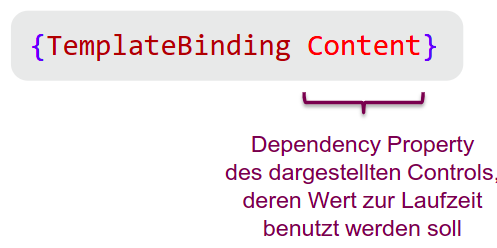
\includegraphics[scale=0.3]{img/template-binding.png}

\subsection{Style Trigger}
Style anhand unterschiedlicher UI-Zustände anpassen
\begin{lstlisting}[language=xml]
<Style x:Key="MyButtonStyle" TargetType="Button"> 
  <Setter Property="Background" Value="White" /> 
  <Setter Property="Foreground" Value="Black" /> 
  <Setter Property="Cursor" Value="Hand" /> 
  <Style.Triggers> 
    <Trigger Property="IsMouseOver" Value="True"> 
      <Setter Property="Background" Value="#2672EC" /> 
      <Setter Property="Foreground" Value="White" /> 
    </Trigger> 
  </Style.Triggers> 
</Style> 
\end{lstlisting}


\subsection{Data Trigger}
(in \code{Style.Triggers} eingebunden, wie vorher. Beispiel: Style ist für ListBoxItem, rote Schrift wenn nicht mehr an Lager (\code{InStock == 0})
\begin{lstlisting}
<DataTrigger Binding="{Binding InStock}" Value="0">
    <Setter Property="Foreground" Value="Red" />
</DataTrigger>
\end{lstlisting}

\subsection{Standardverhalten Überschreiben}
\begin{lstlisting}[language=xml]
<Style x:Key="BaseButtonStyle" TargetType="{x:Type ButtonBase}"> 
  ... 
  <Setter Property="Template"> 
    <Setter.Value> 
      <ControlTemplate.Triggers> 
        ... 
        <Trigger Property="IsMouseOver" Value="true"> 
          <Setter Property="Background" Value="{StaticResource Button.MouseOver.Background}" TargetName="border" /> 
          <Setter Property="BorderBrush" Value="{StaticResource Button.MouseOver.Border}" TargetName="border" /> 
        </Trigger> 
        ... 
      </ControlTemplate.Triggers> 
    </Setter.Value> 
  </Setter> 
</Style>
\end{lstlisting}

\subsection{Transformationen}
\subsubsection{2D Transformation}
\begin{lstlisting}[language=xml]
<ScaleTransform ScaleX="1.5" ScaleY="1.5" />
<RotateTransform Angle="45" CenterX="30" CenterY="12" /> 
<SkewTransform AngleX="-35" AngleY="9" />
<TranslateTransform X="40" Y="-10" /> 
\end{lstlisting}
\subsubsection{Transformationen in Styles}
Normal via Style Setter zu bewerkstelligen
\begin{lstlisting}[language=xml]
<Setter Property="RenderTransform"> 
  <Setter.Value> 
    <RotateTransform Angle="3"></RotateTransform> 
  </Setter.Value> 
</Setter> 
\end{lstlisting}
Un um den Ursprungspunkt/Angelpunkt der Transformation anzugeben
\begin{lstlisting}[language=xml]
<Setter Property="RenderTransformOrigin" Value="0.5,0.5"/> 
\end{lstlisting}

\section{Umgang mit Daten}
\begin{description}
\item[Ohne DataBinding:] Programmierer alles selbst, viel zu umständlich, mühsam und fehleranfällig
\item[Mit DataBinding: ] Lesen/Setzen von Properties erfolgt automatisch.
\begin{itemize}
    \item UI via DataContext und Data Binding-Ausdruck verdrahtet
    \item Zustandsänderung an das gebundene Property wird automatisch synchronisiert (TwoWay-Binding)
    \item kein \code{Name} Attribut mehr nötig
\end{itemize}
\end{description}

\paragraph{Markup Extensions}
\begin{description}
\item[\code{x:Type [Datentyp]}] Liefert angegebene Klasse
\item[\code{x:Static [Pfade]}] Bindet eine Konstante, statische Property, Feld oder Enum
\item[\code{x:Null}] Null Wert
\item[\code{StaticResource [Name]}] Statische Bindung an Ressource
\item[\code{DynamicResource [Name]}] Dynamische Bindung an Ressource
\item[\code{Binding ...}] Data Binding Ausdruck
\item[\code{RelativeSource ... }] Setzt die Data Binding Source auf eine relevanten Bezug im Logical Tree
\item[\code{TemplateBinding ...}] Bindet Wert an Eigenschaft des mittels Template dargestellten Controls
\item[\code{x:Reference ...}] Abk. für \verb+{Binding Elementname=...}+
\end{description}

\subsection{Überblick Syntax}
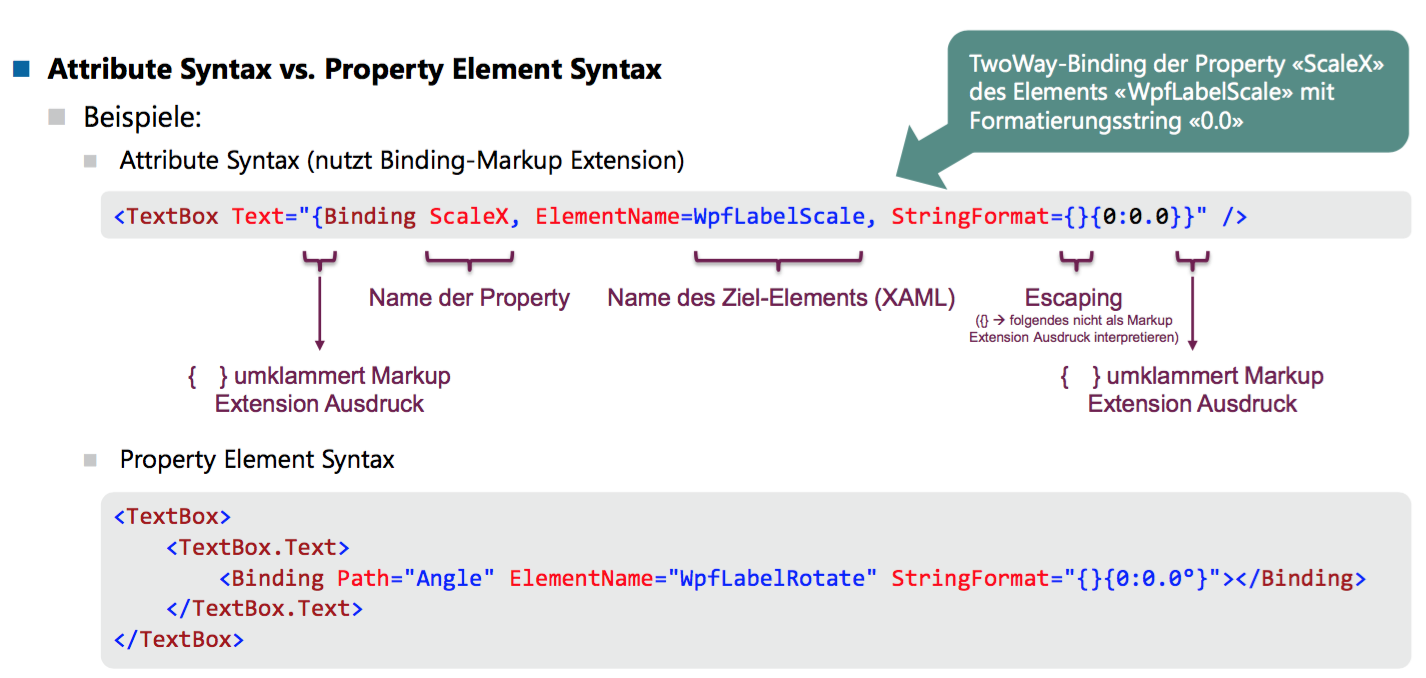
\includegraphics[scale=0.4, angle=90]{DataBinding.png}


\subsection{MultiBinding}
MltiBinding muss mit der Property Syntax gemacht werden:
\begin{lstlisting}[language=xml]
<TextBlock>
  <TextBlock.Text>
    <MultiBinding StringFormat="{}{0} -- Now only {1:0.00}!">
      <Binding Path="Description"/>
      <Binding Path="Price"/>
    </MultiBinding>
  </TextBlock.Text>
</TextBlock> 
\end{lstlisting}


\subsection{Überblick DataBinding}
\paragraph{Voraussetzungen} 
DataContext des Fensters muss auf das Modell gesetzt sein. Die gebundene Model-Klasse muss INotifyPropertyChanged implementieren falls man Änderungnotifikationen haben will.
\paragraph{Binding Base}
\begin{description}
\item[\code{Delay}] Verzögerung in Millisekunden zwischen DataBinding Operation
\item[\code{FallbackValue}] Standardwert, falls Data Binding nicht funktioniert
\item[\code{StringFormat}] Formatierungsangabe für die Umwandlung des Quellwertes in einen String  (für Beispiel siehe MultiBinding oben)
\item[\code{TargetNullValue}] Standardwert, falls Quellwert == null
\end{description}
\paragraph{Binding}
\begin{description}
    \item[\code{BindsDirectlyToSource}] Soll Angabe der Path-Property relativ zum aktuellen Datenprovider (\verb+true+) oder relativ zum Datenkontext (\verb+false+) ausgewertet werden (Nur selten sinnvoll)
    \item[\code{Converter}] Converter der beim Binding benutzt werden soll
    \item[\code{ConverterCulture}] Länderspezifische Einstellungen (\verb+CultureInfo+), welche beim Konvertieren benutzt werden soll
    \item[\code{ConverterParameter}] Zusätzlicher Parameterwert, der dem Converter übergeben werden soll
    \item[\code{ElementName}] Name des XAML-Elements auf welches gebunden werden soll
    \item[\code{Mode}] Richtung des DataBinding (OneTime, OneWay, TwoWay, OneWayToSource)
    \begin{description}
    \item[OneTime:] Eimalig (beim ersten Zugriff)
    \item[OneWay:] Lesend
    \item[TwoWay:] Lesend und Schreibend
    \item[OneWayToSource:] Schreibend
    \end{description}
    \item[\code{Path}] Pfad zur Datenquelle, Objektpfadsyntax
    \item[\code{XPath}] XPath Ausdruck zum Zugriff auf eine XML Datenquelle
    \item[\code{RelativeSource}] Setzt Datenquelle auf Objekt relative zum Ort des aktuellen Elements
    \item[\code{Source}] Setzt Datenquelle
    \item[\code{UpdateSourceTrigger}] Zeitpunkt zu welchem DataBinding getriggert wird
    \begin{description}
        \item[Default] Nutzt festgelegte Trigger der Ziel Property
        \item[Explicit] Nur beim expliziten Aufruf von \verb+UpdateSource()+
        \item[LostFocus] Fokusverlust des Elements
        \item[PropertyChanged] Bei jeder änderung des Inhalts
    \end{description}
\end{description}

\subsection{DataContext, Source, RelativeSource}
Die Datenquelle ist standartmässig nicht gesetzt, muss also explizit gesetzt werden. 

\paragraph{DataContext}
ganzes Fenster via View Model direkt im Code-Behind:
\begin{lstlisting}[language=java]
public partial class MainWindow : Window {
  public MainWindow() {
    InitializeComponent();
    var vm = new PersonViewModel();
    DataContext = vm; 
} }
\end{lstlisting}

\begin{lstlisting}[language=xml]
<TextBlock Text="{Binding FirstName}" />
\end{lstlisting}

ganzes Fenster via ViewModel als Propery im Code-Behind:
\begin{lstlisting}[language=java]
public partial class MainWindow : Window {
  public PersonViewModel MyViewModel { get; set; } // als Property zur Verfügung gestellt
  public MainWindow() {
    InitializeComponent();
    MyViewModel = new PersonViewModel();
    DataContext = MyViewModel;        
} }
\end{lstlisting}

\begin{lstlisting}[language=xml]
<TextBlock Text="{Binding FirstName}" />
\end{lstlisting}

Ganzes Fenster im Code-Behind, aber mit Fenster selbst als View-Model (this)
\begin{lstlisting}[language=java]
public partial class MainWindow : Window { 
  public PersonViewModel MyViewModel { get; set; }
  public MainWindow() {
    InitializeComponent(); 
    MyViewModel = new PersonViewModel();
    DataContext = this;
} }
\end{lstlisting}

\begin{lstlisting}[language=xml]
<TextBlock Text="{Binding MyViewModel.FirstName}" />
\end{lstlisting}

Ganzes Fenster direkt im Code-Behind aber mit Fenster als Liste
\begin{lstlisting}[language=sharpc]
PersonList = new ObservableCollection<PersonViewModel>(list); 
DataContext = this; 
\end{lstlisting}
\begin{lstlisting}[language=xml]
<ListBox ItemsSource="{Binding PersonList}">...</ListBox>
\end{lstlisting}

Direkt im XAML
\begin{lstlisting}[language=xml]
<Window.DataContext>
  <local:PersonViewModel />
</Window.DataContext>
\end{lstlisting}

\paragraph{Source} Ermöglicht die Angabe der Datenquelle direkt im DataBinding Ausdruck. Dieses Property kann auf Ressourcen (Static/Dynamic) oder statische (Static) binden.
\begin{lstlisting}[language=xml]
<!-- falls wir eine eigene String-Table haben und diese als Ressource verfügbar ist --> 
<Label Content="{Binding NameLabelCaption, Source={StaticResource Strings}}" /> 

<!-- falls wir die Beschriftung direkt als String-Ressource definiert haben--> 
<Label Content="{Binding Source={StaticResource MyNameLabelCaption}}" /> 

<!-- zum Vergleich: die bereits bekannte Kurzform mittels StaticResource-Markup Extension --> 
<Label Content="{StaticResource MyNameLabelCaption}" Margin="0,0,0.4,0" /> 
\end{lstlisting}

\paragraph{RelativeSource} 
\begin{itemize}
    \item Ermöglicht die Angabe einer relativen Datenquelle im Visual Tree
    \item Eigene Markup Extension dafür: \code{{RelativeSource ....}}
\end{itemize}

\begin{description}
    \item[\code{FindAncestor}] Sucht übergeordnetes Element des Typs (AncestorType) 
    \item[\code{PreviousData}] Bindet auf das vorhergehende Element (nutzbar z.B. in Collections Delta-Vergleiche) 
    \item[\code{Self}] Bindet auf das Element selbst 
    \item[\code{TemplatedParent}] Bindet auf Element, für welches Control Template gilt (nur innerhalb Template sinnvoll) 
    \item[\code{AncestorLevel}] Gibt Vorgänger-Position an, 1 = erster gefundener Vorgänger, 2 = zweiter, etc. 
    \item[\code{AncestorType}] Typ des zu suchenden Vorgänger-Elements 
\end{description}

\begin{lstlisting}[language=xml]
<Label Content="{Binding RelativeSource={RelativeSource FindAncestor, AncestorType=Window}, Path=Title}" />
\end{lstlisting}


\paragraph{Path} 
\begin{description}
    \item[Path Standard-Property] \code{{Binding Firstname} == {Binding Path=Firstname}}
    \item[\code{{Binding}}] Bindet direkt an Datenquelle selbst (als Ganzes)
    \item[\code{{Binding Address.Street}}] Bindet an Property Street der Property Address der Datenquelle
    \item[\code{{Binding Groups[0].Name}}] Bindet an Name des ersten Objekts in Groups-Auflistung der Datenquelle
\end{description}
\paragraph{Mode}
\begin{description}
    \item[OneTime:] Einmalig (bei erstem Zugriff) 
    \item[OneWay:] Lesend
    \item[TwoWay:] Lesend und schreibend 
    \item[OneWayToSource:] Schreibend 
\end{description}

\paragraph{Binding an anderes Element (Binding Path)}
Mit diesem Code kann man den Inhalt von, z.B. einem TextBlock, an die Eingaben in, z.B. einer Textbox, binden. In diesem Beispiel machen wir dies gleich noch durch ein MultiBinding, der Binding-Ausdruck an sich ist aber allgemeingültig.
\begin{lstlisting}
<TextBox Name="FirstName" />
<TextBox Name="LastName" />
<TextBlock>
    <!-- Anzeige: "FirstName LastName" -->
    <MultiBinding StringFormat="{}{0} {1}">
        <!-- Binden an FirstName.Text -->
        <Binding ElementName="FirstName" Path="Text" />
        <Binding ElementName="LastName" Path="Text" />
    </MultiBinding>
</TextBlock>
\end{lstlisting}

\paragraph{StringFormat}
Umwandeln eines Wertes in einen String (zur Anzeige). Funktioniert auch mit MultiBinding.
\begin{lstlisting}[language=xml]
<TextBox Text="{Binding ScaleX, ElementName=WpfLabelScale, StringFormat={}{0:0.0}}" /> 
\end{lstlisting}

\subsection{Converter}
\paragraph{IValueConverter} Ein Interface welches alle Converter implementieren müssen
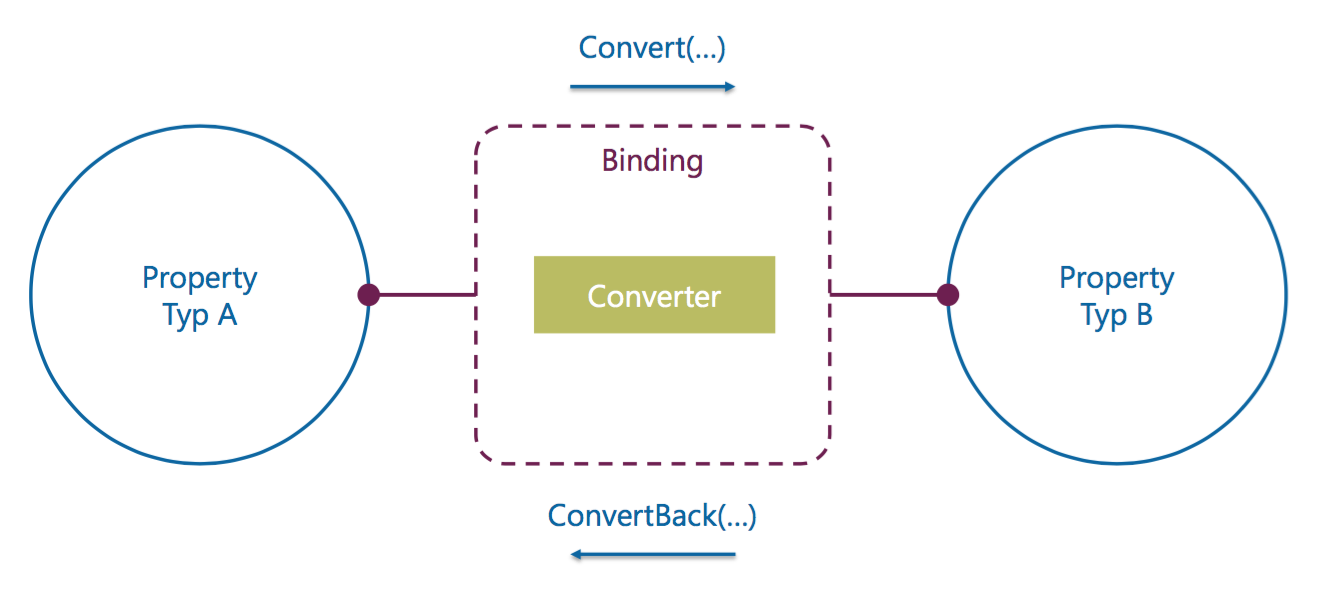
\includegraphics[scale=0.25]{IValueConverter.png}

Es ist auch möglich, nur eine der Methoden zu überschreiben und die andere mit NotImplementedException auszustatten, wenn man es selber nicht verwendet \\
\\
Konvertiert bool oder Nullable in Visibility und zurück
\begin{lstlisting}
public sealed class BooleanToVisibilityConverter: IValueConverter
{
    // value = bool oder nullable, targetType = Visibility
    public object Convert(object value, Type targetType, object parameter, CultureInfo culture)
    {
        return value is bool && (bool)value == true ? Visibility.Visible : Visibility.Collapsed;
    }
    // value = Visibility value, targetType = bool
    public object ConvertBack(object value, Type targetType, object parameter, CultureInfo culture)
    {
        return value as Visibility? == Visibility.Visible
    }
}
\end{lstlisting}
\paragraph{IMultiValueConverter} Konvertiert die Werte der einzelnen Binding-Quellen eines MultiBindings in einen einzelnen Zielwert und umgekehrt. Das Interface dass alle MultiConverter implementieren müssen. Anwendungsbeispiel: Basieren auf einzelnen Farbkomponenten eine Instanz der Color Klasse berechnen resp. die Color Klasse in deren Einzelteile zerlegen.
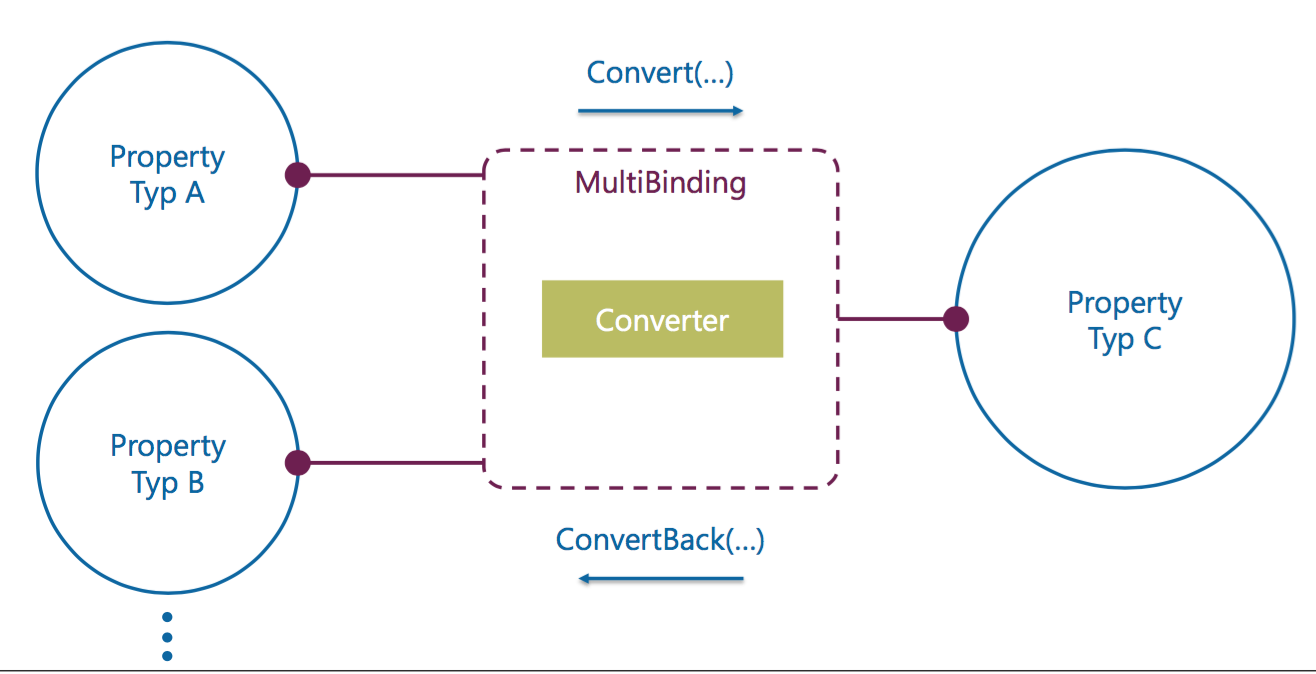
\includegraphics[scale=0.25]{IMultiValueConverter.png}
\begin{lstlisting}
public class RgbToColorConverter: IMultiValueConverter
{
    // values = Werte der binding quelle  
    // Type = Rückgabetyp     parameter = optionaler Parameter um konvertierung genauer zu steuern
    public object Convert(object[] values, Type targetType, object parameter, CultureInfo culture)
    {
        if (values == null)
            return DependencyProperties.Unsetvalue;
        if(values.Length != 3)
            throw new NotSupportedException("3 Values needed)";
        var r = (byte)System.Convert.ToInt32(values[0]);
        var g = (byte)System.Convert.ToInt32(values[1]);
        var b = (byte)System.Convert.ToInt32(values[2]);
        return Color.FromRgb(r,g,b);
    }
    public object[] ConvertBack(object value, Type[] targetType, object parameter, CultureInfo culture)
    {
        if(value == DependencyProperty.UnsetValue)
            return null;
        if(value is Color)
        {
            var color = (Color) value;
            var colors = new object[] {color.R, color.G, color.B};
            return colors;
        }
        return null;
    }
}
\end{lstlisting}
\paragraph{Value Converter anwenden} Um einen Converter anwenden zu können wird eine Instanz benötigt. Instanziierung:
\begin{lstlisting}[language=xml]
<Window.Resources>
    <local:RgbToColorConverter x:Key="MyRgbToColorConverter" />
    <local:BestContrastingColorConverter x:Key="MyBestContrastingColorConverter" />
</Window.Resources>
\end{lstlisting}
Danach kann man den Converter wie gewohnt nutzen:
\begin{lstlisting}
<SolidColorBrush>
    <SolidColorBrush.Color>
        <MultiBinding Converter="{StaticResource MyRgbToColorConverter}">
            <Binding ElementName="ColorR" Path="Value"></Binding>
            <Binding ElementName="ColorG" Path="Value"></Binding>
            <Binding ElementName="ColorB" Path="Value"></Binding>
        </MultiBinding>
    </SolidColorBrush.Color>
</SolidColorBrush>
<SolidColorBrush Color="{Binding Path=Content, ElementName=ColorLabel,
    Converter={StaticResource MyBestContrastingColorConverter}, Mode=OneWay}" />
\end{lstlisting}
Wenn man eigene Value Converters implementiert wird der XAML Code kürzer und man hat eine Entkopplung von Wert und dessen Darstellungseigenschaften. Aber es ist aufwändig und teilweise nicht trivial.



\paragraph{Bindung auf eigene Objekte} 

% Die sogenannten \textbf{DependencyProperties} ermöglichen ein Two-Way Binding und funktionieren mit Key-Value Dictionaries.Sie sind spezialisiert für die Vewendung in einem UI und somit nicht geeignet für Business Objects.
% \begin{lstlisting}
% public int MyProperty
% {
%   get {return (int(GetValue(MyPropertyPropert); }
%   set { SetValue(MyPropertyProperty, value); }
% }
% public static readonly DependencyProperty MyPropertyProperty = 
%     DependencyPropery.Register("MyProperty", 
%             typeof(int), 
%             typeoof(ownerclass), 
%             new PropertyMetadata(0));
% \end{lstlisting}


Mit dem \verb+INotifyPropertyChanged+ Interface können Properties einer Klasse überwacht werden. Das Interface schreibt das Event \verb+PropertyChanged+ vor, das implementiert werden muss. Der Event Handler übermittelt den Namen der geänderten Property.
\begin{lstlisting}
public class PersonV2 : INotifyPropertyChanged {
  public event PropertyChangedEventHandler PropertyChanged;
  // use the name of the calling property if none given:
  private bool SetProperty<T>(ref T field, T value,  [CallerMemberName] string name = null){
    if (Equals(field, value)) { return false; } // basic check for equality...
    field = value;
    PropertyChanged?.Invoke(this, new PropertyChangedEventArgs(name)); 
    return true; 
  } 
  private string _firstName;
  public string FirstName { 
    get { return _firstName; }
    set { SetProperty(ref _firstName, value, nameof(FirstName));
}
 // repeat pattern for other properties... } 
}
\end{lstlisting}
Dies kann auch mit einer Basisklasse gelöst werden, welche die Benachrichtigung implementiert.
\begin{lstlisting}
public abstract class BindableBase: INotifyPropertyChanged
{
    public event PropertyChangedEventHandler PropertyChanged;
    protected bool SetProperty<T>(ref T field, T value, string name = null)
    {
        if(Equals(field,value))
            return false;
        field=value;
        OnPropertyChanged(name);
        return true;
    }
    protected void OnPropertyChanged(string name = null)
    {
        PropertyChanged?.Invoke(this, new PropertyChangedEventArgs(name));
    }
}
public class Person: BindableBase
{
    private string _firstName;
    public string FirstName;
    {
        get { return _firstName; }
        set { SetProperty(ref _firstName, value, nameof(FirstName)); }
    }
}
\end{lstlisting}
\paragraph{Berechnete Properties} Hat man zusammengesetzte Properties, wie zum Beispiel ein FullName, welcher sich aus dem First- und den LastName zusammensetzen, so muss man bei einer Änderung eines Teiles, auch das berechnete Property updates. Das geschieht mit einem Param-Array.
\begin{lstlisting}
protected bool SetProperty<T>(ref T storage, T value, string name, params string[] otherNames)
{
    if(Equals(storage, value))
        return false;
    storage = value;
    OnPropertyChanged(name);
    foreach(var n in otherNames)
        OnPropertyChanged(n);
    return true;
}
\end{lstlisting}

Um das dann zu verwenden, gibt man im Aufruf von SetProperty einfach die berechneten Properties auch noch an, also:
\begin{lstlisting}
private string _lastName;
public string LastName
{
    get { return _lastName; }
    set
    {
        SetProperty(ref _lastName, value, nameof(LastName), 
        nameof(FullName) /*, weitere */);
    }
}
\end{lstlisting}


\paragraph{PropertyChanged.Fody} Fody ist ein Framwork, welches sich in den Kompilationsprozess einhängt und automatisch Properties überwacht. Damit Fody weiss welche Properties er überwachen muss, muss man es mit dem Attribut \verb+ImplementPropertyChanged+ markieren. 


\paragraph{ObservableCollection} Diese Klasse implementiert das \code{INotifyCollectionChanged} und \code{INotifyPropertyChanged} Interface. Diese Collection meldet Änderungen an sich automatisch, somit ist Event Handling auf neue Listeninhalte, bestimmte Positionen oder die gesamte Liste möglich. Aber \textbf{keine} Änderungen an den Inhaltsobjekten selbst, dort ist das \code{INotifyPropertyChanged} nötig.


\paragraph{ItemsControl}
\begin{description}
\item[Basisklasse] von ListBox und ComboBox
\item[Items] Gibt hart codierte Liste von Items an 
\item[ItemsSource] Datenquelle / Data Binding Ausdruck für Items
\item[ItemTemplate] Template für die Darstellung eines Items
\item[ItemTemplateSelector] Selector für das Template eines Items
\end{description}
 

Angabe des Templates direkt im Control
\begin{lstlisting}[language=xml]
<ListBox ItemsSource="{Binding MyTodoList}" HorizontalContentAlignment="Stretch"> 
  <ListBox.ItemTemplate> 
    <DataTemplate> 
      <StackPanel> 
        <TextBlock Text="{Binding TaskName}" /> 
        <TextBlock Text="{Binding Description}"/> 
        <TextBlock Text="{Binding Priority}"/> 
      </StackPanel> 
    </DataTemplate> 
  </ListBox.ItemTemplate> 
</ListBox> 
\end{lstlisting}

Ablage als (wiederverwendbare) Ressource
\begin{lstlisting}[language=xml]
<DataTemplate x:Key="MyTaskTemplate" DataType="local:Task"> 
  <DockPanel HorizontalAlignment="Stretch"> 
    <TextBlock Text="{Binding TaskName}" /> 
    <TextBlock Text="{Binding Description}"/> 
    <TextBlock Text="{Binding Priority}"/> 
  </DockPanel> 
</DataTemplate>

<!-- Verwendung dann via StaticResource -->
<ListBox ItemsSource="{Binding MyTodoList}" ItemTemplate="{StaticResource MyTaskTemplate}" HorizontalContentAlignment="Stretch" /> 
\end{lstlisting}

\paragraph{Selector}
\begin{itemize}
    \item Erbt von ItemsControl
    \item Basisklasse von ListBox, ComboBox, TabControl
\end{itemize}
\begin{description}
    \item[\code{SelectedIndex}] Index des ausgewählten Elements in der Liste 
    \item[\code{SelectedItem}] Ausgewähltes Element selbst (Objekt/ViewModel) 
    \item[\code{SelectedValue}] Bestimmter Property-Wert des ausgewählten Elements 
    \item[\code{SelectedValuePath}] Objektpfadnotation (Name der Property) für Wert, der in SelectedValue zurückgegeben werden soll 
\end{description}

\paragraph{ObjectDataProvider} Ermöglicht Verwendung einer beliebigen Datenquelle mit folgenden Zusatzmöglichkeiten. Es können Parameter an den Konstruktor übergeben werden (ConstructorParameters) oder es können Methoden inkl. Paramter gebunden werden (MethodParameters). Man kann damit beispielsweise Enums auf eine ComboBox binden.
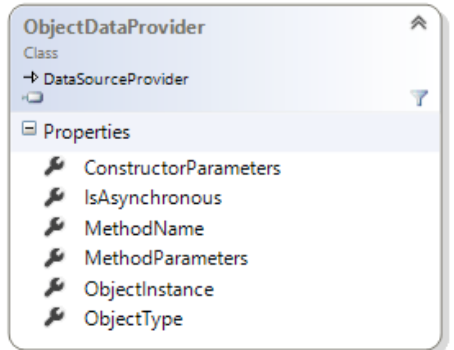
\includegraphics[scale=0.35]{ObjectDataProvider.png}

\begin{lstlisting}[language=xml]
<Window.Resources>
    <ObjectDataProvider x:Key="Alignments"
        MethodName="GetNames"
        ObjectType="{x:Type sys:Enum}">
    <ObjectDataProvider.MethodParameters>
        <x:Type TypeName="VerticalAlignment" />
    </ObjectDataProvider.MethodParameters>
    </ObjectDataProvider>
</Window.Resources>

<!-- Verwendung -->
<ComboBox ItemsSource="{Binding Source={StaticResource Alignments}}" />
\end{lstlisting}
\paragraph{DataBinding Debuggen} Man hat diverse Möglichkeiten die Abläufe hinter dem DataBinding sichtbar zu machen.
\begin{enumerate}
\item Direkt im Binding konfigurieren
\begin{lstlisting}[language=xml]
<!-- System.Diagnostics-Namespace - hinzufuegen -->
xmlns:diag="clr-namespace:System.Diagnostics;assembly=WindowsBase"
<!-- Binding Ausdruck um Setzten des TraceLevels erweitern -->
<TextBlock Text="{Binding ElementName=stack, Path=InvalidPath, diag:PresentationTraceSources.TraceLevel=High}" />
\end{lstlisting}
\item Dummy Converter schreiben
\begin{lstlisting}
public class DebugDummyConverter : IValueConverter
{
    public object Convert(object value, Type targetType, object parameter, CultureInfo culture)
    {
        return value;
    }
    public object ConvertBack(object value, Type targetType, object parameter, CultureInfo culture)
    {
        return value;
    }
}
\end{lstlisting}
\begin{lstlisting}[language=xml]
<Window.Resources> ... <local:DebugDummyConverter x:Key="MyDummy" /> ... </Window.Resources>
...
<TextBlock Text="{Binding ElementName=stack, Path=InvalidPath, Converter={StaticResource MyDummy}}" />
\end{lstlisting}
\item In VisualStudio DataBinding Debugging auf "{}All"{} setzten und im Output-Window nach \verb+Syste.Windows.Data+ suchen.
\end{enumerate}

\subsection{INotifyPropertyChanged (INPC)}
\begin{itemize}
    \item Benötigt bei: \code{OneWay}, \code{TwoWay}
    \item Nicht benötigt bei: \code{OneTime}, \code{OneWayToSource}
\end{itemize}





% \section{CUIT}
% Annahmen: es gibt ein Fenster mit \code{Title="Login Window"}. In diesem Fenster gibt es zwei \code{Textbox}en mit LoginName und Password (Attribut \code{Name=}), und einen \code{Button} der sich LoginButton nennt. Stimmt das Login, so öffnet sich ein Fenster mit dem Titel \code{"Welcome Window"}, welches ein \code{Label} mit dem Namen NameLabel besitzt.

% Wir wollen nun den Usernamen und das Passwort abfüllen, OK klicken, und sehen ob das korrekte Fenster aufgeht.

% \begin{lstlisting}
% [TestClass]
% public class LoginWindowUiTest
% {
%   // Das Folgende kann immer gleich implementiert werden
%   // the directory in which the test is running
%   public string BaseDir => Path.GetDirectoryName(Assembly.GetExecutingAssembly().Location);
%   // system under test (wpf app to be tested)
%   public string SutPath => Path.Combine(BaseDir, $"ch.hsr.wpf.03.login.exe");
  
%   [TestMethod]
%   public void TestMethod1()
%   {
%   var app = Application.Launch(SutPath);
%   var window = app.GetWindow("Login Window", InitializeOption.NoCache);
%   var name = window.Get<TextBox>("LoginName");
%   var pw = window.Get<TextBox>("Password");
%   name.Text = "j.bond";
%   pw.Text = "topsecret";
%   var button = window.Get<Button>("LoginButton");
%   button.Click();
%   var win = app.GetWindow("Welcome Window", InitializeOption.NoCache);
%   var label = win.Get<Label>("NameLabel");
%   Assert.AreEqual("j.bond", label.Text);
%   win.Close();
%   app.Close();
%   }
  
% }
% \end{lstlisting}



\section{MVVM}
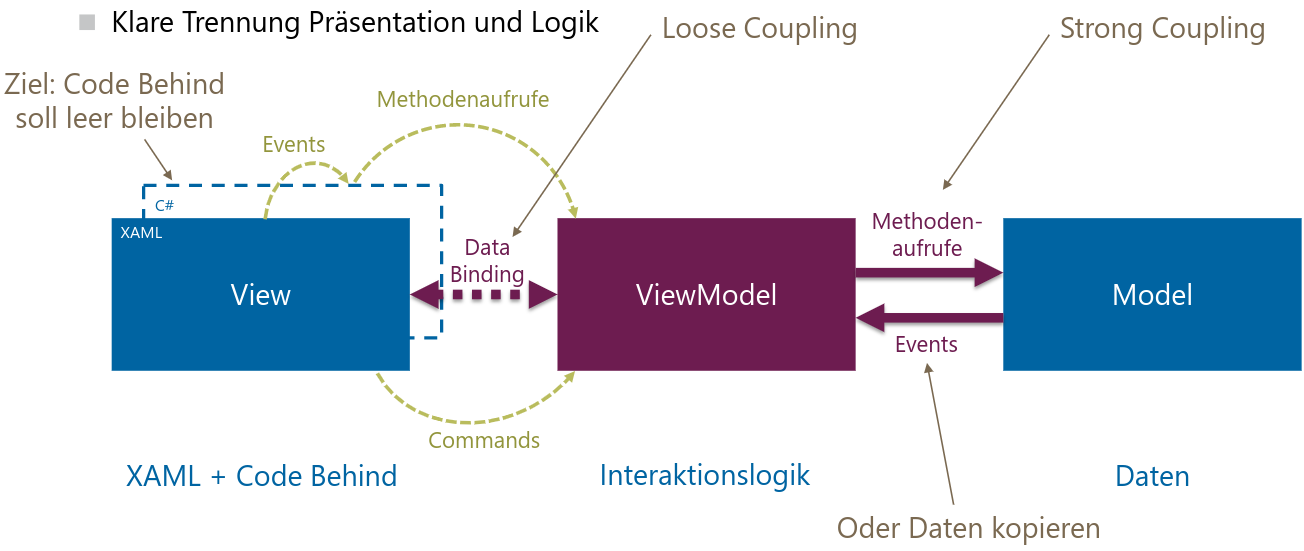
\includegraphics[scale=0.27, angle=90]{img/mvvm_uebersicht.png}

\paragraph{Model} 
\begin{itemize}
    \item Eigentliche Daten
    \item Domain Objekte haben kein Verhalten
    \item Nicht zuständig für: Formatierung, Laden, Speichern
\end{itemize}

\paragraph{ViewModel} 
\begin{itemize}
    \item View-spezifische Objekte, welche die Domain Objekte um Daten, Berechnungen für die View anreichern
    \item ''Butler'' für eine View, präsentiert alles auf dem Silbertablett
    \item Zuständig für die Darstellung und Formatierung der Daten im Hinblick auf die Darstellung der View
    \item Grundlage für stressfreies DataBinding
\end{itemize}
\textbf{Bilanz}
\begin{itemize}
    \item Modelklassen bleiben einfache POCOs
    \item ViewModels teilen via PropertyChanged-Event mit, wenn sich etwas ändert
    \item ViewModels sind somit für DataBindingvorbereitet 
    \item Fleissarbeit (Kopieren von Properties) übernimmt Library (z.B. AutoMapper) 
    \item Aktionen können via Commands ausgelöst werden 
    \item ViewModels sind testbar, da keine direkte Verdrahtung mit UI-Code
\end{itemize}

\paragraph{Zusammenarbeit Model $\Leftrightarrow$ ViewModel}
Ganzes Model als Property kapseln (nützt nur etwas, wenn sich ganzes Model ändert)
\begin{lstlisting}[language=sharpc]
public class GadgetVm:BindableBase { 
  private Gadget _gadget;
  public Gadget Gadget { 
    get { return _gadget; }
    set { SetProperty(ref _gadget, value, nameof(Gadget));
    }
}
//eventuell noch anderer Code
} 
\end{lstlisting}

Für jede im UI benötigte Property eine gleichnamige VM-Property implementieren (Fleissarbeit $\Rightarrow$ automapper verwenden)
\begin{lstlisting}[language=sharpc]
public class GadgetVm:BindableBase 
{ 
  private string _inventoryNumber; 
  public string InventoryNumber 
  { 
    get { return _inventoryNumber; } 
    set { SetProperty(ref _inventoryNumber, value, nameof(InventoryNumber)); } 
  } 
  //eventuell noch anderer Code 
}
\end{lstlisting}

\paragraph{View} 
\begin{itemize}
    \item XAML + Code Behind (wenig)
    \item Zustände via Data Binding zwischenspeichern
    \item Designs: Styles mit Control Templates
    \item Layouts: UserControl
    \item Möglichst so schreiben, dass viele Teile wiederverwendet werden können
    \item Möglichst wenig (am besten kein) Zugriff auf die UI Controls aus dem Code Behind (Thema Kopplung)
    \item Zustände im DataBinding speichern
    \item 
\end{itemize}

%\paragraph{Anmerkung} Auf Interfaces Referenzieren die eine andere Komponente implementiert ist ok.




\subsection{Commands}
\begin{description}
    \item[\code{ICommand}] im ViewModel implementieren und dann via DataBinding auslösen
    \item[Vorteil:] View weiss nichts vom ViewModel und löst nur Aktionen (Commands) aus
    \item[Command] führt die Aktion (z.B speichern) aus
    \item[Command Source] ist das UI-Controls (z.B Button), welcher auf ein Event (z.B Click) reagiert und dann die Aktion (Command) auslöst.
    \item[Command Binding] wird definiert auf dem UI-Control (z.B Button), so dass dieses UI-Control das Kommando beim Event (z.B Klicken) auslöst
\end{description}

\paragraph{Nutzung}
Command werden beim DataBinding wie gewohnt angegeben:
\begin{lstlisting}[language=xml]
<Button Content="Save" Command="{Binding SaveCommand}" /> 
\end{lstlisting}
Falls zusätzliche Parameter übermittelt werden sollen:
\begin{lstlisting}[language=xml]
<Button Content="Open" Command="{Binding OpenGadgetViewCommand}" CommandParameter="{Binding SelectedAuto}" /> 
\end{lstlisting}

\paragraph{Implementierung/Beispiel von Commands}

Eigene Command-Klasse, Instanz davon als Property im ViewModel.
\textbf{Nachteil:} Kein Zugriff auf private Member des ViewModels 
\begin{lstlisting}[language=sharpc]
public class SomeCommand : ICommand { 
  public bool CanExecute(object parameter) { // ... irgendwie true oder false zurückgeben }
  public void Execute(object parameter) { // ... irgendwas ausführen } 
  public event EventHandler CanExecuteChanged;
} 
\end{lstlisting}

\begin{lstlisting}[language=sharpc]
public class GadgetVm:BindableBase { 
  // streng getypt, oder auch nur ICommand:
  public SomeCommand MyCommand { get; set; }
  // public ICommand MyCommand { get; set; } 
  public GadgetVm() {
  MyCommand = new SomeCommand(); 
  } //weiterer Code }
\end{lstlisting}

Command als innere Klasse im ViewModel implementieren.
\textbf{Vorteil} Zugriff auf private Member des ViewModels

\begin{lstlisting}[language=sharpc]
public class GadgetVm:BindableBase // Start des ViewModels {
   ...
   public class SomeCommand : ICommand // Start des Commands { 
     public bool CanExecute(object parameter) { // ... irgendwie true oder false zurückgeben }
     public void Execute(object parameter) { // ... irgendwas ausführen // ... jetzt aber mit Zugriff auf private Members } public event EventHandler CanExecuteChanged;
     private GadgetVm ViewModel { get; set; } 
     // eine Instanz auf das ViewModel übergeben:
     public SomeCommand(GadgetVm vm) { ViewModel = vm; } 
   } // Ende des Kommandos ... 
} // Ende des ViewModels 
     
\end{lstlisting}

\subsection{RelayCommand}
''Command-Pattern'', das man selber implementieren muss, aber dann viel Zeit und Geld spart (Ziit und Geld han ich kei).

Nicht-generic RelayCommand
\begin{lstlisting}
public class RelayCommand : ICommand
{
    private readonly Action _execute;
    private readonly Func<bool> _canExecute;
    
    public RelayCommand(Action execute, Func<bool> 
        canExecute = null)
    {
        if (execute == null) throw new 
            ArgumentNullException("execute");
        
        _execute = execute;
        _canExecute = canExecute;
    }
    
    public bool CanExecute(object parameter) => 
        _canExecute?.Invoke() ?? True
    public void Execute(object parameter) => _execute();
    
    // Event an CommandManager delegieren (Benachrichtigung erfolgt
    // so immer dann wenn WPF denkt, dass sich etwas am Ausführungs- 
    // status geändert hat, z.B. bei Key- oder Mouse-Button-Klick)
    public event EventHandler CanExecuteChanged
    {
        add { CommandManager.RequerySuggested += value; }
        remove { CommandManager.RequerySuggested += value }
    }
}
\end{lstlisting}

Die Generic-Variante nutzt ein \mintinline{csharp}{Action<T>} als \mintinline{csharp}{_execute} und ein \mintinline{csharp}{Predicate<T>} als \mintinline{csharp}{_canExecute}

Verwendung:

\begin{lstlisting}
public class GadgetVm : BindableBase
{
    public ICommand SaveCommand { get; set; }
    
    public GadgetVm()
    {
        SaveCommand = new RelayCommand(
            () => this.Save(), // Methode des ViewModels
            () => this.CanSave // Property des ViewModels
        );
    }
    
    public CanSave => ; // some condition
    public void Save() {} // some method
}
\end{lstlisting}

\subsection{ViewModel vs View}
\begin{itemize}
    \item ViewModel kennt die View nicht
    \begin{itemize}
    \item Keine Referenz auf die View
    \item Falls Parameter benötigt: als CommandParamter übergeben oder Klassen-intern cachen
    \item ViewModel erstellt die View nicht selbst 
    \end{itemize}
    \item View kennt ViewModel auch nicht
    \begin{itemize}
        \item Keine Referenz auf das ViewModel (ausser DataContext)
        \item Verbindung zu Datenelementen und Commands nur deklarativ via Data Binding
    \end{itemize}
    \item ViewModel und View werden ''von aussen'' erzeugt.
    \item ViewModel wird ''von aussen'' als DataContext für die View gesetzt
\end{itemize}


\subsection{StartupCode} Wer erstellt VMs, Vs und lädt Ms? Spezielles AppVM verwenden, welches beim Start erzeugt wird. Zusätzliche VMs werden vom APPVM erzeugt (Factory). Views werden direkt innerhalb der View erzeugt. VM erzeugt, lädt und speichert Ms

\begin{lstlisting}
// App.xaml Startup Uri entfernen

// App Class
public AppVm {get; set; }
protected override void onStartup(StartupEventArgs e)
{
  base.OnStartup(e);
  AppVm = new AppVm
    
    // hier: eine der Varianten unten
}

// V1: Internes Erzeugen  
MainWindow = new MainView();
MainWindow.Show();

public GadgeothekView() { 
  InitializeComponent();
  DataContext = new GadgetVm(); } 


// V2: Dependency Injection (via Property)
var vm = new ViewModel();
MainWindow = MainView();
MainView.DataContext = vm;
MainWindow.Show();

public GadgeothekView() { InitializeComponent(); }

// V3: Dependency Injection via Konstruktor
var vm = new GadgetVm(); 
MainWindow = new GadgeothekView(vm);
MainWindow.Show();

public GadgeothekView(GadgetVm vm) { 
  InitializeComponent();
  DataContext = vm; } 

\end{lstlisting}
\section{Architekturthemen}

\subsection{Dependency Injection}
\begin{itemize}
    \item View-Models in einem X-Plattform-Projekt haben keinen Zugriff auf UI-Komponenten und können somit:
    \begin{itemize}
        \item keine Fenster öffnen
        \item keine UI Events direkt behandeln
        \item generell keine platformspezifischen Dinge erledigen
    \end{itemize}
    \item Um das dennoch zu machen $\Rightarrow$ Dependency Injection
\end{itemize}

Wie erreichen wir den Zugriff auf plattformspezifischen Code?
\begin{enumerate}
    \item Wir abstrahieren den Zugriff mittels Interface
\begin{lstlisting}
public interface INavigationService 
{ 
  void Show(string view, object vm); 
} 
\end{lstlisting}
    \item Wir programmieren im ViewModel-Code gegen diese Interfaces
\begin{lstlisting}
public class AutoListVm : BindableBase {
  // Service in Property speichern
  public INavigationService NavigationService { get; }
  //Service im Konstruktor übergeben
  public AutoListVm(INavigationService navService) { 
    // Service der Propery zuweisen
    NavigationService = navService;
  } 
  public void ShowDetailView() {
    // Service verwenden
    NavigationService.Show("Auto", SelectedAuto); 
} } 
\end{lstlisting}
    \item Wir implementieren im Plattform-Projekt für jedes abstrakte Interface einen konkreten Service
\begin{lstlisting}
// Service Klasse
public class WpfNavigationService : INavigationService 
{ 
  public readonly Dictionary<string, Action<object>> WindowFactory = new Dictionary<string, Action<object>>(); 
  
  public WpfNavigationService() 
  { 
    WindowFactory.Add("AutoList", vm => AutoListWindow.Display(vm as AutoListVm)); 
    WindowFactory.Add("Auto", vm => AutoWindow.Display(vm as AutoVm)); 
    WindowFactory.Add("Customer", vm => CustomerWindow.Display(vm as CustomerVm)); 
  } 
  public void Show(string view, object vm) 
  { 
    var factoryAction = WindowFactory[view];
    factoryAction(vm); 
  } 
} 
\end{lstlisting}
    \item Wir instanziieren die verwendeten Service im Startup-Code des Plattform-Projekts
    \item Wir injizieren den ViewModels die beötigten Services (z.B via Konstruktor-Parameter)
\begin{lstlisting}
public partial class App : Application 
{ 
  public AppVm Vm { get; private set; } 
  public INavigationService NavigationService { get; private set; } 
  protected override void OnStartup(StartupEventArgs e) 
  { 
    base.OnStartup(e); 
    NavigationService = new WpfNavigationService(); 
    Vm = new AppVm(NavigationService); 
    ... 
  }
} 
\end{lstlisting}
\end{enumerate}
\paragraph{Verbesserungmöglichkeiten}
Anstatt Magic-String wie etwa ''AutoList'' zu verwendet, können folgende bessere Wege verwendet werden:
\begin{enumerate}
    \item String-Konstanten 
    \item Enums
    \item Typ-Parameter (Generics)
\end{enumerate}
Die dritte Variante ist empfohlen:

\begin{lstlisting}
public interface INavigationService { void Show<T>(T vm); }

public class WpfNavigationService : INavigationService { 
  public readonly Dictionary<Type, Action<object>> WindowFactory = new Dictionary<Type, Action<object>>();
  public WpfNavigationService() { 
    WindowFactory.Add(typeof(AutoListVm), vm => AutoListWindow.Display(vm as AutoListVm)); WindowFactory.Add(typeof(AutoVm), vm => AutoWindow.Display(vm as AutoVm)); 
    WindowFactory.Add(typeof(CustomerVm), vm => CustomerWindow.Display(vm as CustomerVm)); } 
    public void Show<T>(T vm) {
      var factoryAction = WindowFactory[typeof(T)];
      factoryAction(vm);
} } 
\end{lstlisting}


\paragraph{Vorteile / Nachteile}
\begin{itemize}
    \item[+]  Zwang zur ''Separation of Concerns'' 
    \item[+] Konfigurierbare Lebensdauer von Objekten 
    \item[+] Konfigurierbare Multiplizität von Objektinstanzen (z.B. Singleton, Object-Pool) 
    \item[+] Flexiblere Testbarkeit (Mock-Services) 
    \item[+] Einfacherer Austausch einer Service-Implementierung durch eine andere 
    \item[-] Konfigurationsfehler fallen erst zur Laufzeit auf 
    \item[-] (Scheinbar) höhere Komplexität 
    \item[-] Mehr Code 
    \item[-] Code wird (un)übersichtlicher
    \item[-] Dadurch Code auch schwieriger zu debuggen
\end{itemize}


\subsection{Background Execution}
Standardmässig laufen 2 Threads:
\begin{description}
    \item[UI-Thread] Event Handling, Layout Management
    \item[Render-Thread] Zeichnen der Controls auf den Screen
\end{description}
\begin{itemize}
    \item Fenster werden neu gezeichnet auch während einer ''Blockade''
\end{itemize}

\paragraph{Tasks}
\begin{lstlisting}
Task.Run(() =>
{
    // Anwendung im Background
    // UI-Thread läuft parallel weiter
});
\end{lstlisting}

\paragraph{Dispatcher}
\\
Synchron
\begin{lstlisting}
Dispatcher.Invoke(() =>
{
    // UI blockiert
});
\end{lstlisting}
Asynchron
\begin{lstlisting}
Dispatcher.BeginInvoke(() =>
{
    // UI nicht blockiert
});
\end{lstlisting}


\subsection{Background Operation}
\begin{enumerate}
    \item Visuelles Feedback geben (Spinner, Overlay, Popup)
    \item Starten eines BG-Threads, Kontrolle geht gleich an UI Thread zurück
    \item Bei Thread-Ende aus dem BG-Thread den UI-Thread irgendwie benachrichtigen
\end{enumerate}
\begin{lstlisting}
public void CreateAsciiArtinBackgroundThread()
{
    Task.Run(() =>
    {
        // Berechnung läuft nun in einem Background Thread
        CreateAsciiArt();
        // am Schluss den Dispatcher nutzen, um eine abschliessende Aktion im UI-Thread auszuführen: 
        Dispatcher.Invoke(() => { ... });
    });
}
\end{lstlisting}





\section{Benutzerinteraktion}
\paragraph{Routed Events}
\begin{itemize}
    \item Interessante UI Ereignisse, auf die reagieren soll (Mouse, Keyboard oder Touch-Ereignisse)
    \item Routed Events können mit \code{Handled = "True"} unterbrochen/abgebrochen werden
    \item 2 Phasen: abwärts (Preview/Tunnelling) und dann aufwärts (Bubbeling) gerouted (wie bei HTML 5) 
    \item Preview Event wird vor dem eigentlichen Event ausgeführt (hier kann man prüfen, ob z.B die gedrückte Taste eine Nummer war)
\end{itemize}
% 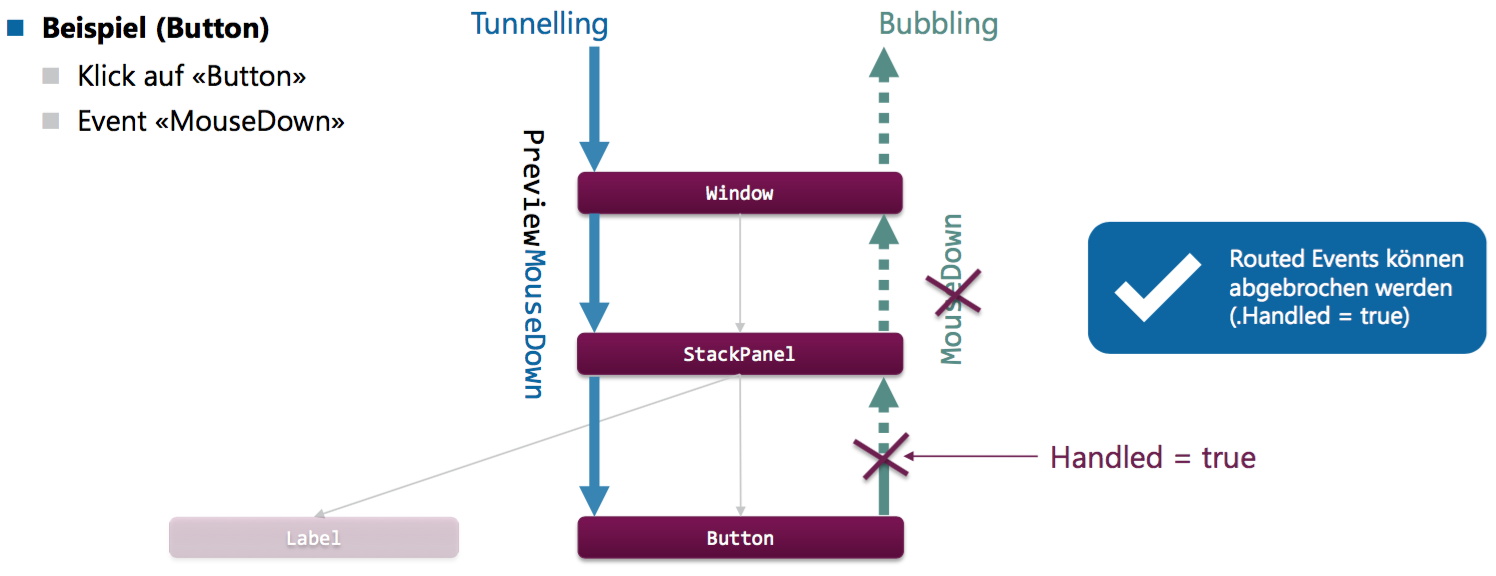
\includegraphics[scale=0.25]{RoutedEvent1.png}
% 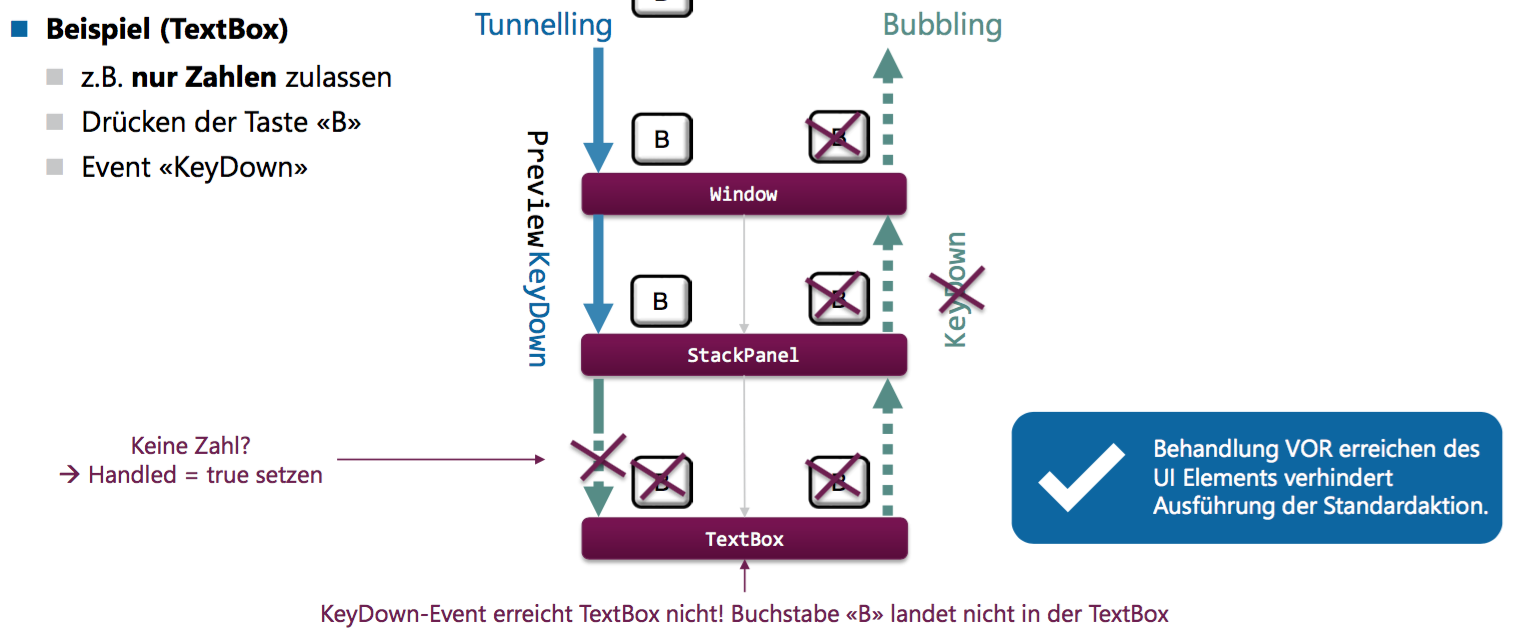
\includegraphics[scale=0.25]{RoutedEvent2.png}
UI Events können beim Ui Element selbst behandelt werden:
\begin{lstlisting}[language=xml]
<Button Name="SaveButton"
    PreviewMouseDown="SaveButton_OnPreviewMouseDown"
    MouseDown="SaveButton_OnMouseDown">Save</Button>
\end{lstlisting}


Oder beim Parent Element
\begin{lstlisting}[language=xml]
<StackPanel PreviewMouseDown="StackPanel_OnPreviewMouseDown">
    ...
    <Button Name="SaveButton"
        PreviewMouseDown="SaveButton_OnPreviewMouseDown"
        MouseDown="SaveButton_OnMouseDown">Save</Button>
    ...
</StackPanel>
\end{lstlisting}


Eine andere Alternative wäre mit Attached Events.
\begin{lstlisting}[language=xml]
<StackPanel Button.Click="StackPanel_OnClick">
    ...
    <Button Name="SaveButton" Click="SaveButton_OnClick">Save</Button>
    ...
</StackPanel>
\end{lstlisting}

Routed Events behandeln im Code Behind: \\
Grundlegend wenn UI Control einen Namen hat (Zugriff wie gewohnt)
\begin{lstlisting}
private void SaveButton_OnPreviewMouseDown(object sender, MouseButtonEventArgs e) { 
// Dinge prüfen, bevor das Event das Element erreicht hat } 
private void SaveButton_OnMouseDown(object sender, MouseButtonEventArgs e) { //Event behandeln } 
\end{lstlisting}
Geht auch wenn das UI Control keinen Namen hat (UI Control einen Namen geben und casten):
\begin{lstlisting}
private void SaveButton_OnMouseDown(object sender, MouseButtonEventArgs e) { 
var saveButton = sender as Button; }
\end{lstlisting}

\textbf{Beliebte Mouse Events:}
\begin{tabular}{ll}
MouseDown & MouseEnter* \\
MouseLeave* & MouseLeftButtonDown \\
MouseLeftButtonUp & MouseMove \\
MouseRightButtonDown & MouseRightButtonUp \\
MouseUp & MouseWheel
\end{tabular}

\textbf{Interessante Keyboard Events:} \\
\begin{tabular}{ll}
KeyDown & KeyUp \\
TextInput & 
\end{tabular}

\textbf{Interessante Touch-Events:} \\
\begin{tabular}{ll}
TouchDown & TouchEnter* \\
TouchLeave* & TouchMove \\
TouchUp & 
\end{tabular}
\\
* \textit{haben kein Preview Event}


\paragraph{RoutedEventArgs} RoutedEventArgs leiten von EventArgs ab. 
\begin{description}
\item[\code{Handled}] Boolean der aussagt, ob das Event behandelt wurde
\item[\code{OriginalSource}] Quell-Element (Hit-Testing) welches das Event ausgelöst hat
\item[\code{RoutedEvent}] Das RoutedEvent, welches mit diesem Objekt verknüpft ist
\item[\code{Source}] Element, welches das Event rapportiert hat
\end{description}

Die OriginalSource kann ein Kind-Element des Source-Elements sein, das per Hit-Testing als 1. Adressat des Events bestimmt wurde. Die Source ist das Element im Logical Tree, welches das Event rapportiert hat. Beispielsweise beim Subscribe auf MouseDown auf einem Button, wird das Event vom Button rapportiert (Source), wurde aber eigentlich vom Rahmen ausgelöst (OriginalSource).

\paragraph{Ableitende Klasse von RoutedEventArgs} Es gibt für verschiedene Input-Geräte Ableitungen von RoutedEventArgs. Auswahl von \verb+MouseEventArgs+:
\begin{itemize}
\item \textbf{LeftButton}: Zustand der linken Maustaste (Pressed/Released)
\item \textbf{MiddleButton}
\item \textbf{RightButton}
\item \textbf{Delta}: Mausradbewegung (-120/120)
\end{itemize}
Auswahl von \verb+KeyEventArgs+:
\begin{itemize}
\item \textbf{Key}: Taste (Enum)
\item \textbf{IsDown}
\item \textbf{IsUp}
\item \textbf{IsRepeat}
\item \textbf{SystemKey}: Die zusätzliche Taste, falls ALT-Taste gedrückt wurde. Key steht in \verb+Key.System+
\end{itemize}
\subsection{Drag \& Drop}
Drag \& Drop besteht aus 3 Phasen:
\begin{enumerate}
\item \textbf{Maustaste wird gedrückt:} Nach überschreiten einer Mindestdistanz wird die Aktion gestartet
\item \textbf{Während des Ziehens:} Steuerelemente unterhalb des Zeigers müssen melden, ob sie als Ziel infrage kommen
\item \textbf{Fallenlassen:} Steuerelement unterhalb des Mauszeigers muss eine Aktion mit dem bewegten Objekt durchführen
\end{enumerate}
Beispiel:
\begin{lstlisting}
public ObservableCollection<UserInfo> AvailableUsers { get; set; }
public ObservableCollection<UserInfo> SelectedUsers { get; set; }
public MainWindow()
{
    // Listen initialisieren und fuellen
    InitializeComponent();
    DataContext = this;
}
\end{lstlisting}
\paragraph{Phase 1} Maustaste wird gedrückt
\begin{lstlisting}[language=xml]
<ListBox Name="AvailableListBox" ItemsSource="{Binding AvailableUsers}"
    ItemTemplate="{StaticResource UserInfoTemplate}"
    PreviewMouseLeftButtonDown="AvailableListBox_ OnPreviewMouseLeftButtonDown"
    PreviewMouseLeftButtonUp="AvailableListBox_ OnPreviewMouseLeftButtonUp"
    MouseMove="AvailableListBox_OnMouseMove" />
\end{lstlisting}
\begin{lstlisting}
private Point? dragStartPosition = null;
private void AvailableListBox_ OnPreviewMouseLeftButtonUp(object sender, MouseButtonEventArgs e)
{
    dragStartPosition = null;
}
private void AvailableListBox_ OnPreviewMouseLeftButtonDown(object sender, MouseButtonEventArgs e)
{
    dragStartPosition = e.GetPosition(this);
}
private bool IsMovementFarEnough(Point origPos, Point curPos)
{
    var minDistX = SystemParameters.MinimumVerticalDragDistance;
    var minDistY = SystemParameters.MinimumHorizontalDragDistance;
    return (Math.Abs(curPos.X - origPos.X) >= minDistX || Math.Abs(curPos.Y - origPos.Y) >= minDistY);
}
private void AvailableListBox_OnMouseMove(object sender, MouseEventArgs e)
{
    // gar nicht starten, wenn nicht (innerhalb Liste) geklickt
    if (dragStartPosition == null)
        return;
    // aktuelle Position holen und pruefen, ob die Maus genug
    // bewegt wurde, um die Bewegung als Drag zu interpretieren
    var position = e.GetPosition(this);
    if (!IsMovementFarEnough(dragStartPosition.Value, position))
        return;
    // Alles ok, drag kann starten
    dragStartPosition = null;
    StartDrag(AvailableListBox.SelectedItem as UserInfo);
}
private void StartDrag<T>(T obj)
{
    // Bereich definieren, auf dem der Drag-Vorgang gueltig ist
    var dragScope = this.Content as FrameworkElement;
    // Container fuer Nutzdaten (hier String)
    var dragData = new DataObject(typeof(T), obj);
    // Drag-Vorgang starten
    DragDrop.DoDragDrop(dragScope, dragData, DragDropEffects.Move);
}
\end{lstlisting}
Die \verb+DragDrop.DoDragDrop+ Methode blockiert die weitere Code-Ausführun bis die Operation beendet ist.
\paragraph{Phase 2} Maus wird gezogen
\begin{lstlisting}[language=xml]
<ListBox Name="SelectedListBox" ItemsSource="{Binding SelectedUsers}"
    ItemTemplate="{StaticResource UserInfoTemplate}"
    AllowDrop="True"
    DragOver="SelectedListBox_OnDragOver"
    Drop="SelectedListBox_OnDrop" />
\end{lstlisting}
\begin{lstlisting}
private void SelectedListBox_OnDragOver(object sender, DragEventArgs e)
{
    // Objekt auspacken
    var data = e.Data.GetData(typeof(UserInfo)) as UserInfo;
    // falls Objekt verfuegbar, dann kopieren, sonst keine Operation
    e.Effects = data != null ? DragDropEffects.Copy : DragDropEffects.None;
}
\end{lstlisting}
\paragraph{Phase 3} Objekt wird fallengelassen
\begin{lstlisting}[language=xml]
<ListBox Name="SelectedListBox" ItemsSource="{Binding SelectedUsers}"
    ItemTemplate="{StaticResource UserInfoTemplate}"
    AllowDrop="True"
    DragOver="SelectedListBox_OnDragOver"
    Drop="SelectedListBox_OnDrop" />
\end{lstlisting}
\begin{lstlisting}
private void SelectedListBox_OnDrop(object sender, DragEventArgs e)
{
    // Objekt auspacken
    var user = e.Data.GetData(typeof(UserInfo)) as UserInfo;
    // Dank Data Binding reicht es nun, das UserInfo Objekt
    // der ObservableCollection hinzuzufuegen:
    SelectedUsers.Add(user);
}
\end{lstlisting}
\paragraph{Drag \& Drop Events}
\begin{description}
\item[DragEnter] Tritt auf, wenn dieses Element während einer Drag-Operation als Drag Target fungieren würde (Hit-Testing)
\item[DragLeave] Tritt auf, wenn dieses Element während einer Drag-Operation verlassen wird
\item[DragOver] Tritt auf, wenn diesem Element eine Drag-Operation stattfindet
\item[Drop] Tritt auf, wenn das Objekt der Drag-Operation auf dieses Element fallengelassen wird
\item[GiveFeedback] Gibt der Quelle der Drag-Operation eine Chance, visuelles Feedback zu geben
\end{description}


\paragraph{ColorSlider}
\begin{lstlisting}
// MainWindow.xaml
ValueChanged="ColorSlider_ValueChanged"
// MainWindow.xaml.cs
private void ColorSlider_ValueChanged(object sender, RoutedPropertyChangedEventArgs<double> e)
{
	var r = (byte)ColorR.Value;
	var g = (byte)ColorG.Value;
	var b = (byte)ColorB.Value;

	TextR.Text = r.ToString();
	TextG.Text = g.ToString();
	TextB.Text = b.ToString();
	
	var color = Color.FromRgb(r,g,b);
	ColorArea.Fill = new SolidColorBrush(color);
	ColorLabel.Content = color.ToHexColor(false);
}
\end{lstlisting}
\paragraph{Normal Click Event}
\begin{lstlisting}[language=xml]
<!-- MainWindow.xaml -->
<StackPanel Margin="240,120,0,0">
	<TextBlock Name="Greeting" Text="{Binding Greeting}" FontSize="48" FontFamily="Segoe UI Light"   Margin="0,0,0,40" />
	<TextBlock Text="What's your name?" FontSize="16" FontFamily="Segoe UI Light" />
	<StackPanel Orientation="Horizontal" Margin="0,20,0,20" >
		<TextBox Name="NameInput" Text="{Binding Name}" Width="300" FontSize="16" 		 VerticalContentAlignment="Center" FontFamily="Segoe UI" BorderThickness="0" 		 HorizontalAlignment="Left" Margin="0,0,10,0"/>
		<Button Name="SayHelloButton" Content="Say &quot;Hello&quot;" FontSize="16" FontFamily="Segoe UI Light" 	Background="#0065A3" BorderThickness="2" BorderBrush="White" Foreground="White" 	Padding="4" IsDefault="True" Click="SayHelloButton_Click" />
	</StackPanel>
</StackPanel>
\end{lstlisting}
\begin{lstlisting}
// MainWindow.xaml.cs
private void SayHelloButton_Click(object sender, RoutedEventArgs e){
	Greeting.Text = $"Hello, {NameInput.Text}!";
}
\end{lstlisting}

\end{multicols*}
\end{document}
